\documentclass[10pt,a4paper]{article}
\usepackage[T1]{fontenc}
\usepackage[utf8]{inputenc}
\usepackage{lmodern,microtype}
\usepackage[margin=24mm]{geometry}
\usepackage{float,graphicx,booktabs,longtable,array,calc,etoolbox}
\usepackage{tikz}
\usepackage{amsmath,amssymb}
\usepackage{caption}
\usepackage[numbers,sort&compress]{natbib}
\usepackage{xurl}
\usepackage[hidelinks]{hyperref}
\usepackage{bookmark}
\setlength{\emergencystretch}{3em}
\setlength{\parskip}{4pt}
\setlength{\parindent}{0pt}
\setlength{\tabcolsep}{4pt}
\AtBeginEnvironment{longtable}{\small}
\captionsetup{font=small,labelfont=bf}
\providecommand{\tightlist}{\setlength{\itemsep}{0pt}\setlength{\parskip}{0pt}}
\let\originalappendix\appendix
\renewcommand{\appendix}{\originalappendix\numberwithin{table}{section}}
\newcommand{\pandocbounded}[1]{#1}
\title{Tablets and Vnodes During Cluster Expansion and Contraction in ScyllaDB\\[5pt]\large An instrumented single-host comparative case study}
\author{Giorgi Gogsadze\\\small Department of Computer Science, Kutaisi International University, Georgia}
\date{24 September 2026}
\begin{document}
\maketitle
\begin{abstract}
Cluster expansion and contraction couple replica placement, storage maintenance and foreground service. We examine these interactions through one tablet lifecycle and one vnode lifecycle in ScyllaDB on a resource-constrained laptop. Each RF=2 dataset contained 750,000 deterministic rows and traversed a three-to-four-to-three-node sequence. The treatments executed identical sequences of 1.08 million measured operations at a target of 500 operations/s, with zero reported workload failures. Tablets split from 32 to 64 ranges and merged back, achieving equal four-node token-space shares while changing some final replica assignments. Client backlog was largest during tablet expansion and several minutes after vnode contraction; the latter coincided with synchronized deferred storage work. Topology quiescence preceded this delayed slowdown, illustrating the need to evaluate placement and service separately. An offline SSTable audit accounted for all 72,501 excess final vnode entries as overlap across local files: exactly 750,000 distinct keys remained, each on two nodes. Together, these findings connect placement transitions, maintenance and physical accounting. Unequal baselines, asymmetric log retention and one lifecycle per treatment constrain causal and statistical generalization.
\end{abstract}
\textbf{Keywords:} ScyllaDB; tablets; virtual nodes; topology changes; streaming; compaction; measurement validity
\hypertarget{introduction}{%
\section{Introduction}\label{introduction}}

Adding a database node starts a sequence of changes. The cluster updates membership, moves replicas and reclaims obsolete files. Meanwhile, clients keep sending requests as the storage engine reorganizes data. Removing a node creates a similar coordination problem. Topology metadata can look settled while clients and disks remain busy. Operation latency or command-return time alone can miss that unfinished work.

ScyllaDB offers two ways to distribute data: vnode-based token ownership and table-specific tablets with explicit replica placement \cite{r1,r6}. This allows a comparison within the same database implementation, schema, replication factor and workload. Reading the measurements requires care, however. Tablet replica sizes, vnode ownership percentages, stream-manager byte counters and SSTable partition estimates each describe a different part of the system.

This paper follows a complete expansion/contraction lifecycle to answer three questions. How do placement and observed quiescence evolve? How do client scheduling, operation latency and storage maintenance relate to those changes? Which apparent differences remain after checking metric definitions, sampling and physical storage contents?

The investigation aligns request logs with topology changes and resource activity. Retained vnode server logs, source code from the exact build and an offline audit of preserved SSTables help explain the resulting patterns. Together, these records reconstruct tablet placement inheritance, connect delayed work to client disruption and resolve an apparent excess of physical replicas. The result is a baseline comparison of scaling mechanisms under constrained resources.

\hypertarget{background-and-related-work}{%
\section{Background and related
work}\label{background-and-related-work}}

Distributing data starts with a placement rule. Dynamo assigns multiple virtual positions to each physical node so the system can redistribute data incrementally \cite{r24}. Apache Cassandra documents the balance and operational tradeoffs of multiple tokens, including a larger set of replica neighbors \cite{r29}. Equal token counts therefore need not give nodes equal replicated ownership. Bigtable takes a range-based approach, managing tablets independently \cite{r25}. ScyllaDB partitions each table's replicated token space and assigns its tablets explicitly to hosts and shards \cite{r1}.

ScyllaDB's implementation account describes tablets as units of placement and storage organization \cite{r27}. Each tablet has associated memtables and SSTables, and migration includes cleanup. Its Raft-topology account explains how a fault-tolerant topology coordinator coordinates metadata changes \cite{r28}. These mechanisms motivate tracking both range boundaries and replica assignments. Both treatments in this study use the same ScyllaDB build. Cassandra studies supply context for the comparison, while the experiment examines data distribution within ScyllaDB itself.

Elasticity research asks what changing capacity costs while a database serves requests. Kuhlenkamp, Klems and Röss compare Cassandra and HBase using scaling speed and workload impact \cite{r30}. They also examine how infrastructure and reproduction affect results. Yamaguchi and Morimitsu identify disk I/O during Cassandra node joining as a bottleneck and investigate page-cache and I/O-scheduling changes \cite{r31}. Their findings motivate examining storage activity alongside topology. They do not establish the cause of a slowdown in this experiment.

OnlineElastMan uses workload prediction and a learned performance model to provision Cassandra storage under changing load and response-time objectives \cite{r32}. It studies proactive capacity control. Our fixed, externally triggered lifecycle complements that work by tracing the immediate and delayed effects of each change.

YCSB provides a configurable framework for cloud-serving evaluation \cite{r26}. Our custom serial client preserves identical operation/key sequences and records both scheduled and actual starts. This makes accumulated backlog directly auditable.

Storage files offer a second way to check the measurements. ScyllaDB aggregates SSTable estimates when reporting partition counts \cite{r21}. A key can appear in multiple local files, so the sum can exceed the number of distinct replicas. Flushing writes memtables to disk while leaving other aspects of memory state intact \cite{r5}. We therefore track logical ownership, physical file overlap, maintenance and client service separately.

\newpage

\hypertarget{experimental-design}{%
\section{Experimental design}\label{experimental-design}}

\hypertarget{testbed-and-controls}{%
\subsection{Testbed and controls}\label{testbed-and-controls}}

\begin{longtable}[]{@{}
  >{\raggedright\arraybackslash}p{(\columnwidth - 2\tabcolsep) * \real{0.2600}}
  >{\raggedright\arraybackslash}p{(\columnwidth - 2\tabcolsep) * \real{0.7400}}@{}}
\caption{Experimental configuration and available hardware evidence.}\label{tab:setup}\tabularnewline
\toprule\noalign{}
\begin{minipage}[b]{\linewidth}\raggedright
Component
\end{minipage} & \begin{minipage}[b]{\linewidth}\raggedright
Configuration
\end{minipage} \\
\midrule\noalign{}
\endfirsthead
\toprule
Component & Configuration \\
\midrule
\endhead
\bottomrule\noalign{}
\endlastfoot
Host & Windows laptop, 16 GB RAM; Docker-managed Linux VM \\
Processor & Intel Core i5-13450HX, x86-64; 1 socket, 10 cores (6
performance + 4 efficient), 16 logical processors \\
Nominal clocks & Base speed shown by Windows: 2.40 GHz; manufacturer maximum
turbo 4.60 GHz \cite{r34} \\
Storage & NVMe SSD, SOLIDIGM SSDPFINW010TZL \\
VM allocation evidence & Approximately 9.711 GiB displayed as the common
Docker memory ceiling in both treatments; configured memory and vCPU
limits unavailable \\
Database & ScyllaDB 2026.3.0-0.20260828.10c95df28f74 \\
Per-node settings & Two shards, \texttt{-\/-memory\ 2G}, developer mode,
overprovisioned \\
Topology & One datacenter, one rack; initially three nodes \\
Replication & NetworkTopologyStrategy, RF=2, durable writes \\
Treatments & Tablets enabled; tablets disabled with 256 vnodes per
node \\
Schema & \texttt{id\ bigint\ PRIMARY\ KEY,\ value\ text} \\
Storage settings & IncrementalCompactionStrategy;
LZ4WithDictsCompressor; caching ALL \\
Dataset & 750,000 IDs, 0-749,999; deterministic 1,024-character values;
seed 42 \\
Workload & One synchronous client; target 500 operations/s; 80\%
reads \\
Consistency & LOCAL\_QUORUM for reads and writes \\
\end{longtable}

I checked the processor and SSD model after the experiments. Windows reported a base speed of 2.40 GHz, with virtualization enabled. I did not record effective CPU frequency, storage throughput or the VM's configured vCPU and memory limits during the runs. The maximum turbo frequency comes from the manufacturer specification \cite{r34}. Docker displayed a common, rounded memory ceiling of 9.711 GiB. Two Scylla shards and \texttt{--memory 2G} describe database process settings. They do not establish the VM's vCPU count or a container hard-memory quota.

The exact version and build ID match ScyllaDB's published x86-64 \textbf{release} entry \cite{r33}. The date/commit suffix identifies that release build; it does not mark a pre-release. Developer mode is a separate runtime setting. The schema and LOCAL\_QUORUM settings follow ScyllaDB's documented interfaces \cite{r2,r3}.

Each treatment started with fresh project-scoped volumes and a distinct keyspace. Tablets ran first on 21 September 2026; vnodes followed on 22 September. Fixed container names and network addresses required sequential execution. The dataset stayed loaded throughout each lifecycle. Checks, warmups and operator delays separated the workload phases, so mixed traffic did not run continuously across the entire day.

RF=2 gives a three-node baseline meaningful placement choices. The single-rack tablet configuration falls outside ScyllaDB's RF-rack-valid terminology \cite{r10}. A separate keyspace-creation warning also reported RF below the recommended threshold of three. The system still permits the placement and streaming observations studied here. The findings apply to this single-rack warning state; the experiment did not test rack failures.

Startup warnings establish further limits on the testbed. The perf-event stall detector fell back to a timer, and SCHED\_FIFO scheduling was unavailable. ScyllaDB reported approximately 974 MiB per shard and an improperly configured I/O scheduler. These departures from recommended deployment conditions matter when interpreting performance \cite{r7}.

\newpage

\hypertarget{lifecycle-and-workload-matching}{%
\subsection{Lifecycle and workload
matching}\label{lifecycle-and-workload-matching}}

\begin{longtable}[]{@{}
  >{\raggedright\arraybackslash}p{(\columnwidth - 10\tabcolsep) * \real{0.14}}
  >{\raggedright\arraybackslash}p{(\columnwidth - 10\tabcolsep) * \real{0.1}}
  >{\raggedleft\arraybackslash}p{(\columnwidth - 10\tabcolsep) * \real{0.12}}
  >{\raggedleft\arraybackslash}p{(\columnwidth - 10\tabcolsep) * \real{0.1}}
  >{\raggedleft\arraybackslash}p{(\columnwidth - 10\tabcolsep) * \real{0.12}}
  >{\raggedright\arraybackslash}p{(\columnwidth - 10\tabcolsep) * \real{0.38}}@{}}
\caption{Measured lifecycle phases; each phase is preceded by a read-only warmup.}\label{tab:lifecycle}\tabularnewline
\toprule\noalign{}
\begin{minipage}[b]{\linewidth}\raggedright
Phase
\end{minipage} & \begin{minipage}[b]{\linewidth}\raggedright
Nodes
\end{minipage} & \begin{minipage}[b]{\linewidth}\raggedleft
Duration (s)
\end{minipage} & \begin{minipage}[b]{\linewidth}\raggedleft
Operations
\end{minipage} & \begin{minipage}[b]{\linewidth}\raggedleft
Seed
\end{minipage} & \begin{minipage}[b]{\linewidth}\raggedright
Topology action
\end{minipage} \\
\midrule\noalign{}
\endhead
\bottomrule\noalign{}
\endlastfoot
Baseline & 3 & 120 & 60,000 & 20260921 & None \\
Expansion & 3 to 4 & 900 & 450,000 & 20260922 & Add node at scheduled
+120 s \\
Four-node & 4 & 120 & 60,000 & 20260923 & None \\
Contraction & 4 to 3 & 900 & 450,000 & 20260924 & Decommission at
scheduled +120 s \\
Final three & 3 & 120 & 60,000 & 20260925 & None \\
\end{longtable}

After loading and verifying each fresh dataset, I flushed the target
table on all three initial nodes before baseline measurement. I did not
deliberately clear caches or restart the surviving nodes between phases.
The later vnode cleanup described below also changed the memtable and
SSTable state.

Every phase began with a 30-second, read-only warmup at the same target rate. The measured workloads selected IDs uniformly and generated deterministic updates. All 1,080,000 corresponding operation-type/ID pairs matched between treatments. All eight recorded source hashes also agreed. Write-state checks compared successful writes with the saved latest expected seeds. Each treatment ended with 186,933 distinct written IDs in its tracked set.

Two procedural differences affected the histories. I repeated the vnode expansion warmup after an initially slower run and excluded both warmups from measured results. I also ran cleanup serially on the original vnode nodes after measured expansion and before the four-node phase. Tablets received no equivalent manual cleanup. The vnode cleanup changed the storage state that subsequent phases inherited.

The study contains one independently initialized lifecycle per treatment. Individual requests provide observations within those lifecycles, not independent treatment replications. The analysis therefore reports descriptive statistics without treatment-level significance tests.

\begin{figure}[H]
\centering
\resizebox{\textwidth}{!}{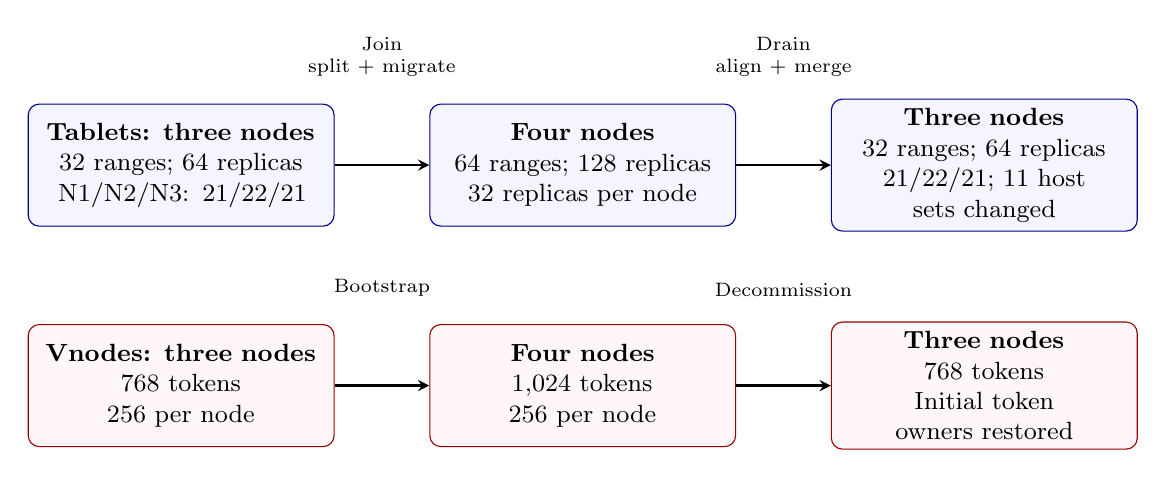
\begin{tikzpicture}[>=stealth,box/.style={draw=blue!55!black,rounded corners,fill=blue!4,text width=3.65cm,minimum height=1.55cm,align=center,font=\small},vbox/.style={box,draw=red!60!black,fill=red!3}]
\node[box] (a) at (0,0) {\textbf{Tablets: three nodes}\\32 ranges; 64 replicas\\N1/N2/N3: 21/22/21};
\node[box] (b) at (5.1,0) {\textbf{Four nodes}\\64 ranges; 128 replicas\\32 replicas per node};
\node[box] (c) at (10.2,0) {\textbf{Three nodes}\\32 ranges; 64 replicas\\21/22/21; 11 host sets changed};
\draw[->,thick] (a)--node[above,yshift=10mm,font=\scriptsize,align=center]{Join\\split + migrate}(b);
\draw[->,thick] (b)--node[above,yshift=10mm,font=\scriptsize,align=center]{Drain\\align + merge}(c);
\node[vbox] (d) at (0,-2.8) {\textbf{Vnodes: three nodes}\\768 tokens\\256 per node};
\node[vbox] (e) at (5.1,-2.8) {\textbf{Four nodes}\\1,024 tokens\\256 per node};
\node[vbox] (f) at (10.2,-2.8) {\textbf{Three nodes}\\768 tokens\\Initial token owners restored};
\draw[->,thick] (d)--node[above,yshift=10mm,font=\scriptsize]{Bootstrap}(e);
\draw[->,thick] (e)--node[above,yshift=10mm,font=\scriptsize]{Decommission}(f);
\end{tikzpicture}}
\caption{Observed membership and range organization. Replica counts count host/shard assignments at RF=2; arrows summarize transitions that included migration. The return to 32 tablet boundaries preserved aggregate counts but changed 11 host sets. Vnode token-owner signatures returned to their initial state.}\label{fig:topology}
\end{figure}

\newpage

\hypertarget{measurement-definitions}{%
\subsection{Measurement definitions}\label{measurement-definitions}}

\textbf{Client operation latency} measures monotonic elapsed time inside the workload's operation boundary. That boundary includes client-side value generation and the driver call. It also includes read validation or expected-write-state handling. The metric therefore combines client work with the database interaction, rather than isolating server execution time.

\textbf{Scheduled-start lag} measures how far the client falls behind its schedule: actual monotonic start offset minus scheduled offset. The client executes operations serially. At 500/s, each operation and its intervening work have a two-millisecond average budget. When they exceed that budget, backlog accumulates; faster execution later allows the client to catch up. The target does not create independent concurrent arrivals or guarantee exactly 500 requests in every wall-clock second.

\textbf{Placement-and-counter quiescence onset} identifies a quiet window in the recorded topology and counters. It is the earliest saved topology observation followed by at least 60 seconds of unchanged placement and idle collected streaming counters, with complete required groups. We identify the onset retrospectively, once the full confirmation window is available. Collection cadence limits its temporal resolution. The criterion covers the recorded metadata and counters; it does not measure all transfer paths, deferred compaction or sustained client recovery.

\textbf{Ownership} measures logical token-space coverage. \textbf{Replica-size bytes} describe reported tablet replica storage. \textbf{SSTable entry counts} count entries in files, while \textbf{distinct local keys} distinguish keys after deduplication. Gross Docker network and block I/O are rounded cumulative values that include other traffic and storage work \cite{r12}. Throughout, MB denotes decimal megabytes; MiB and GiB denote binary units.

\hypertarget{instrumentation-and-analysis}{%
\subsection{Instrumentation and
analysis}\label{instrumentation-and-analysis}}

The collectors tracked the cluster at several timescales. Tablet placement and size sampling ran approximately once per second. Vnode ring commands ran approximately every two seconds and saved raw output, acquisition start/end times and SHA-256 hashes. Another collector recorded the documented incoming/outgoing stream-manager counters per node, shard and direction at roughly one-second intervals \cite{r11}. Docker samples were typically three to four seconds apart. Event records marked command starts, returns and process removal. Separate health checks recorded membership, tasks, streams, restarts and OOM flags.

Phase summaries use linear-interpolated quantiles at position \texttt{(n-1)p}, rounded to three decimals. UTC timestamps align independently recorded evidence. Monotonic fields support duration and scheduling conclusions. Appendix~\ref{measurement-and-evidence-audit} details the clock, sampling and parser checks.

The investigation also checks what the files actually contain. A partition estimate can look excessive when several SSTables hold the same local key. To test that explanation for the final \texttt{tablestats} counts \cite{r4}, we mounted preserved vnode volumes read-only. We used the matching \texttt{dump-statistics} and \texttt{dump-data} tools \cite{r23}. The inventory and modification times identified 12 SSTables corresponding to the pre-shutdown checkpoint. We compared metadata row counts with extracted keys, deduplicated keys within each node and counted node membership for every key. This retrospective audit covers the selected files and excludes later shutdown files and memtables.

\newpage

\hypertarget{results}{%
\section{Results}\label{results}}

\hypertarget{integrity-and-foreground-operation-times}{%
\subsection{Integrity and foreground operation
times}\label{integrity-and-foreground-operation-times}}

Each treatment completed 1.08 million measured operations with zero reported failures, invalid IDs or index errors. Read/write counts matched exactly in phase order: 48,170/11,830; 360,305/89,695; 48,012/11,988; 360,268/89,732; and 48,084/11,916. Saved write-state checks found no missing or mismatched latest seeds. Both treatments ended with 750,000 logical rows. At LOCAL\_QUORUM, checks of 500 written and 500 never-written sampled values per treatment also passed. These checks cover the measured operations and sampled keys.

The comparison starts with an important difference: vnodes already had a lower baseline read p95. Their 2.240 ms compares with 3.033 ms for tablets, approximately \textbf{26.1\% lower}. Baseline lag p95 also differed: 0.006 versus 0.190 s. Matching request sequences therefore did not produce equivalent starting performance. The runs took place in a fixed order on separate days, with different cache and maintenance histories and shared-host activity. Windows available memory later fell to 161 MiB during tablet expansion, but the evidence cannot isolate its effect. The following phase comparisons describe these recorded histories.

\begin{longtable}[]{@{}
  >{\raggedright\arraybackslash}p{(\columnwidth - 12\tabcolsep) * \real{0.2}}
  >{\raggedleft\arraybackslash}p{(\columnwidth - 12\tabcolsep) * \real{0.1333}}
  >{\raggedleft\arraybackslash}p{(\columnwidth - 12\tabcolsep) * \real{0.1333}}
  >{\raggedleft\arraybackslash}p{(\columnwidth - 12\tabcolsep) * \real{0.1333}}
  >{\raggedleft\arraybackslash}p{(\columnwidth - 12\tabcolsep) * \real{0.1333}}
  >{\raggedleft\arraybackslash}p{(\columnwidth - 12\tabcolsep) * \real{0.1333}}
  >{\raggedleft\arraybackslash}p{(\columnwidth - 12\tabcolsep) * \real{0.1333}}@{}}
\caption{Client operation latency by measured phase. All values are
milliseconds; T denotes tablets and V denotes vnodes. Each row
summarizes one run segment, not a replicated treatment estimate.
\label{tab:1}}\tabularnewline
\toprule\noalign{}
\begin{minipage}[b]{\linewidth}\raggedright
Treatment / phase
\end{minipage} & \begin{minipage}[b]{\linewidth}\raggedleft
Read mean
\end{minipage} & \begin{minipage}[b]{\linewidth}\raggedleft
Read p95
\end{minipage} & \begin{minipage}[b]{\linewidth}\raggedleft
Read p99
\end{minipage} & \begin{minipage}[b]{\linewidth}\raggedleft
Write mean
\end{minipage} & \begin{minipage}[b]{\linewidth}\raggedleft
Write p95
\end{minipage} & \begin{minipage}[b]{\linewidth}\raggedleft
Write p99
\end{minipage} \\
\midrule\noalign{}
\endfirsthead
\toprule\noalign{}
\begin{minipage}[b]{\linewidth}\raggedright
Treatment / phase
\end{minipage} & \begin{minipage}[b]{\linewidth}\raggedleft
Read mean
\end{minipage} & \begin{minipage}[b]{\linewidth}\raggedleft
Read p95
\end{minipage} & \begin{minipage}[b]{\linewidth}\raggedleft
Read p99
\end{minipage} & \begin{minipage}[b]{\linewidth}\raggedleft
Write mean
\end{minipage} & \begin{minipage}[b]{\linewidth}\raggedleft
Write p95
\end{minipage} & \begin{minipage}[b]{\linewidth}\raggedleft
Write p99
\end{minipage} \\
\midrule\noalign{}
\endhead
\bottomrule\noalign{}
\endlastfoot
T / Baseline & 1.809 & 3.033 & 3.989 & 1.413 & 2.410 & 3.098 \\
T / Expansion & 1.950 & 3.493 & 4.840 & 1.458 & 2.604 & 3.417 \\
T / Four-node & 1.896 & 3.213 & 4.015 & 1.474 & 2.461 & 3.065 \\
T / Contraction & 1.622 & 2.771 & 3.764 & 1.202 & 2.024 & 2.729 \\
T / Final three & 1.769 & 3.035 & 3.830 & 1.402 & 2.385 & 2.918 \\
V / Baseline & 1.362 & 2.240 & 2.832 & 1.098 & 1.800 & 2.293 \\
V / Expansion & 1.655 & 2.830 & 3.826 & 1.228 & 2.134 & 2.792 \\
V / Four-node & 1.584 & 2.823 & 3.712 & 1.150 & 1.941 & 2.448 \\
V / Contraction & 1.954 & 3.425 & 4.709 & 1.385 & 2.470 & 3.110 \\
V / Final three & 1.826 & 3.153 & 4.005 & 1.355 & 2.323 & 2.896 \\
\end{longtable}

\begin{figure}[H]
\centering
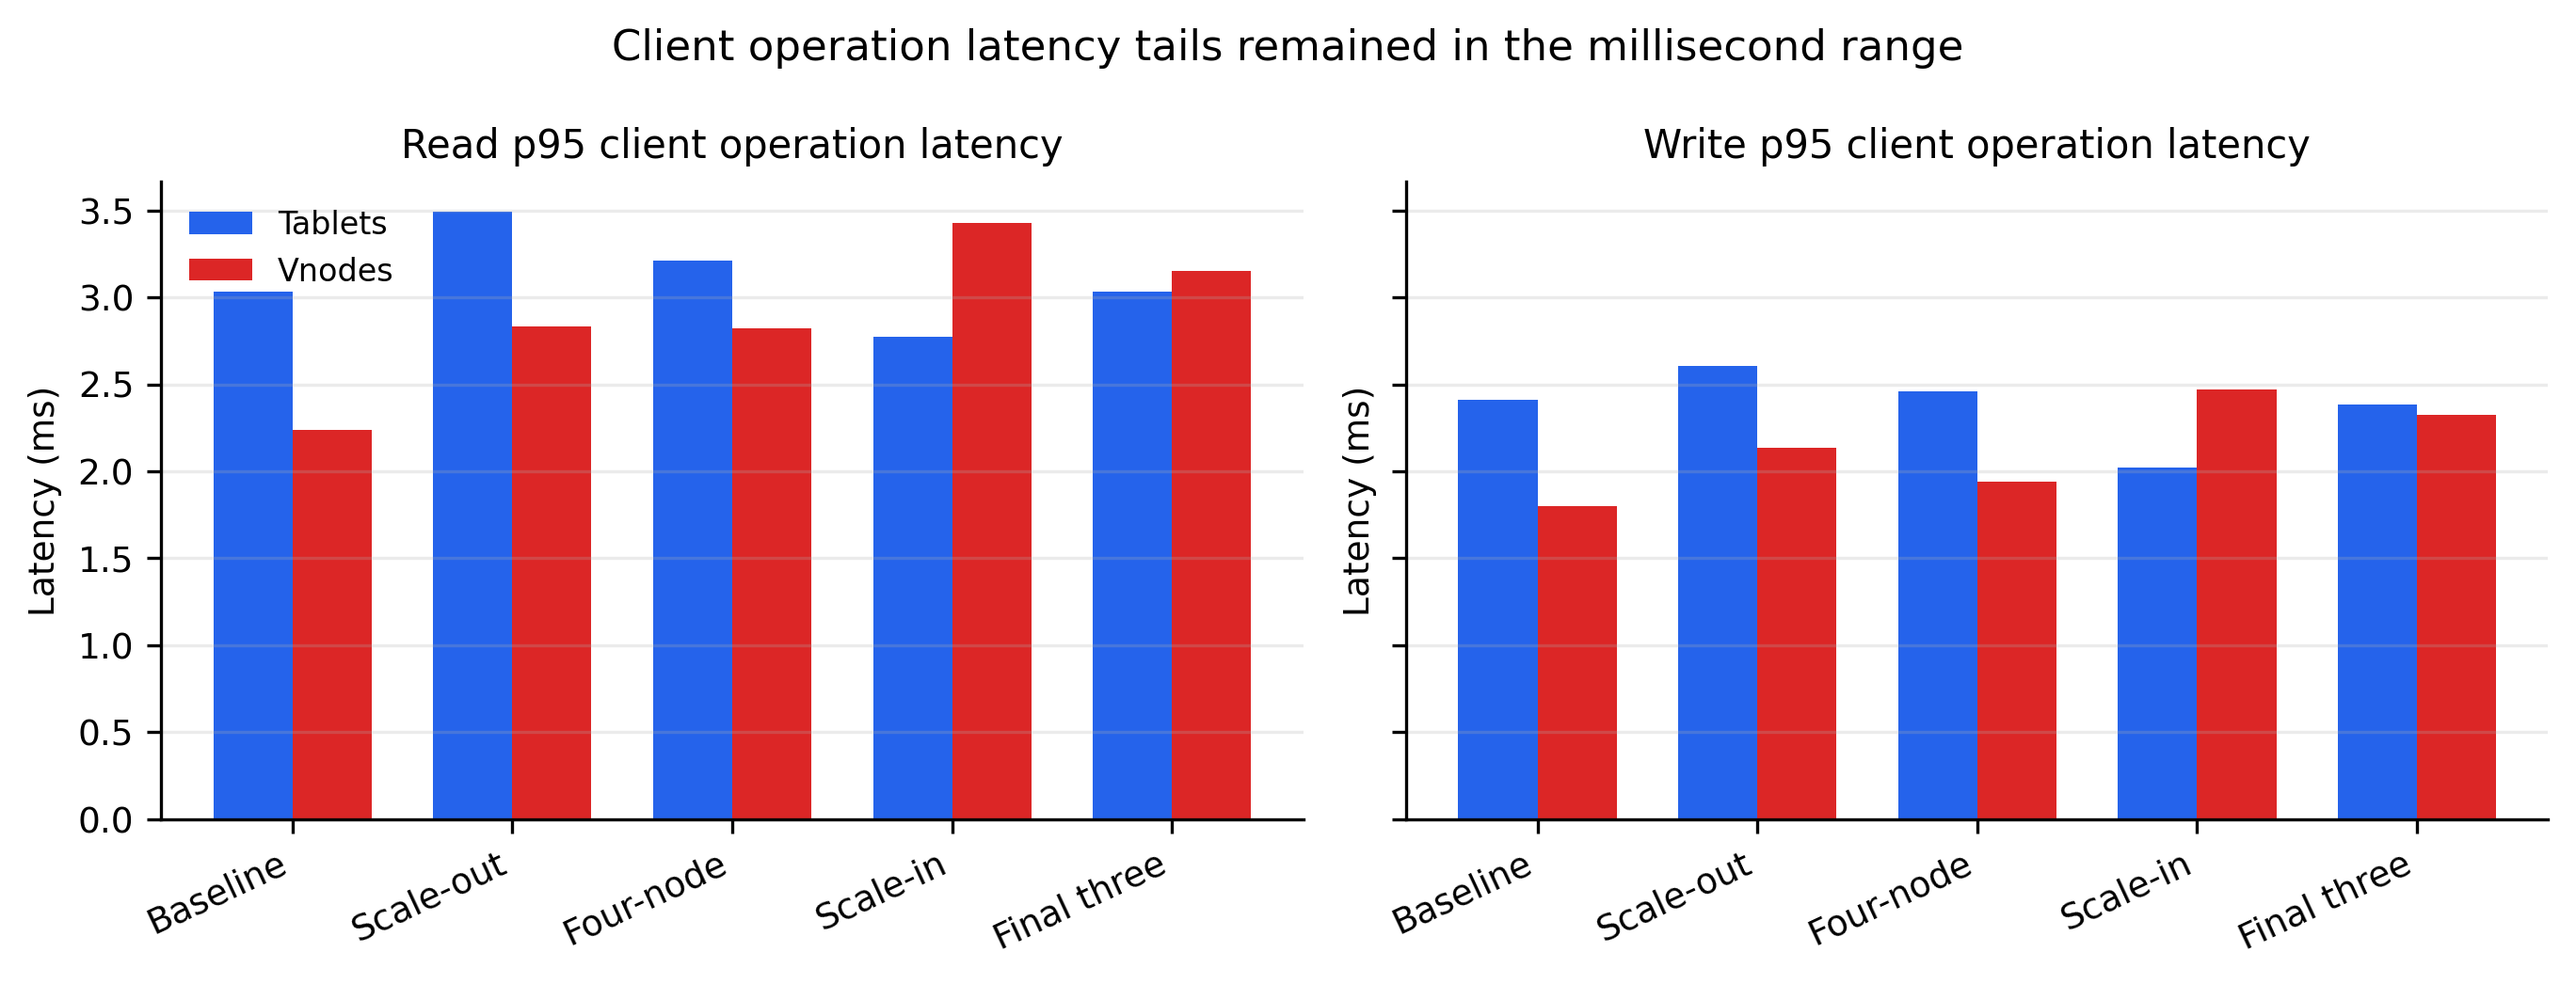
\includegraphics[width=\textwidth,height=.56\textheight,keepaspectratio]{figures/figure_1_phase_latency_p95.png}
\caption{Read and write p95 client operation latency. Millisecond-scale operation times can coexist with seconds of scheduled-start lag because the client issues operations serially.}\label{fig:figure_1_phase_latency_p95}
\end{figure}

Vnodes had lower read p95 values in the first three phases. Tablets had the lower value during contraction, and the final-three read p95 values were close. These observations describe how the two runs behaved. Cache state, maintenance, treatment order and host activity remain intertwined with the choice of data distribution.

\newpage

\hypertarget{placement-quiescence-and-topology-timing}{%
\subsection{Placement quiescence and topology
timing}\label{placement-quiescence-and-topology-timing}}

\begin{longtable}[]{@{}
  >{\raggedright\arraybackslash}p{(\columnwidth - 6\tabcolsep) * \real{0.2000}}
  >{\raggedleft\arraybackslash}p{(\columnwidth - 6\tabcolsep) * \real{0.2667}}
  >{\raggedleft\arraybackslash}p{(\columnwidth - 6\tabcolsep) * \real{0.2667}}
  >{\raggedleft\arraybackslash}p{(\columnwidth - 6\tabcolsep) * \real{0.2667}}@{}}
\caption{Command execution and placement-and-counter quiescence are
distinct endpoints. Trigger lateness is relative to the first measured
request plus 120 seconds. \label{tab:2}}\tabularnewline
\toprule\noalign{}
\begin{minipage}[b]{\linewidth}\raggedright
Transition
\end{minipage} & \begin{minipage}[b]{\linewidth}\raggedleft
Command duration (s)
\end{minipage} & \begin{minipage}[b]{\linewidth}\raggedleft
Quiescence onset (s after command start)
\end{minipage} & \begin{minipage}[b]{\linewidth}\raggedleft
Trigger lateness (s)
\end{minipage} \\
\midrule\noalign{}
\endfirsthead
\toprule\noalign{}
\begin{minipage}[b]{\linewidth}\raggedright
Transition
\end{minipage} & \begin{minipage}[b]{\linewidth}\raggedleft
Command duration (s)
\end{minipage} & \begin{minipage}[b]{\linewidth}\raggedleft
Quiescence onset (s after command start)
\end{minipage} & \begin{minipage}[b]{\linewidth}\raggedleft
Trigger lateness (s)
\end{minipage} \\
\midrule\noalign{}
\endhead
\bottomrule\noalign{}
\endlastfoot
Tablet expansion & 1.584 & 51.265 & 0.214 \\
Vnode expansion & 1.486 & 22.566 & 0.187 \\
Tablet contraction & 15.544 & 17.691 & 0.112 \\
Vnode contraction & 9.932 & 11.323 & 0.159 \\
\end{longtable}

\begin{figure}[H]
\centering
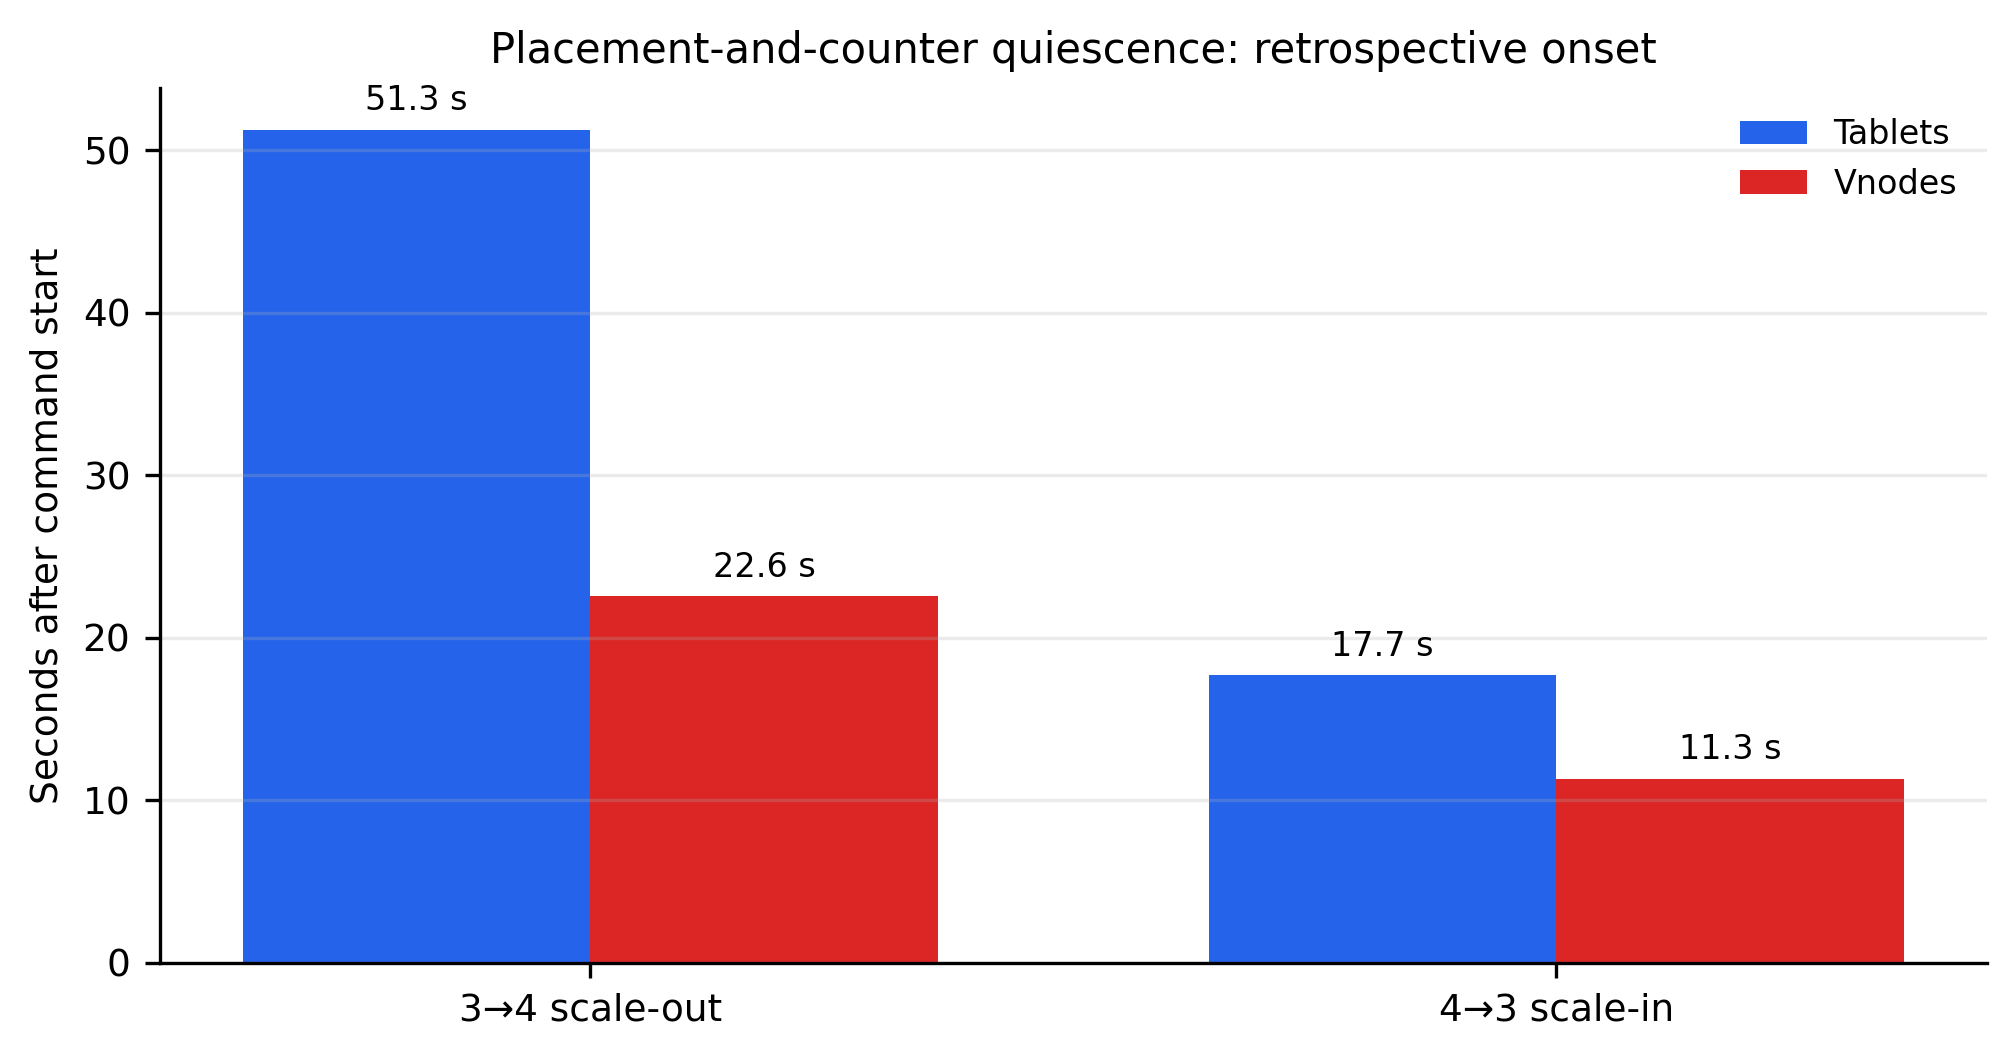
\includegraphics[width=\textwidth,height=.56\textheight,keepaspectratio]{figures/figure_2_convergence_onset.png}
\caption{Earliest sampled start of a subsequently verified 60-second unchanged-placement and idle-counter window. The observations are bounded by collection cadence and counter scope.}\label{fig:figure_2_convergence_onset}
\end{figure}

Vnodes reached the placement-and-counter milestone earlier in both transitions. The contraction result shows why that milestone needs context: vnodes reached it at about 11 seconds, yet their largest client backlog developed roughly five minutes later. The tablet counters also leave part of file transfer unobserved (Section~\ref{movement-observability-differs-by-path}). We therefore interpret these onsets alongside the service and storage results.

The vnode ring first showed a joining fourth node, then all 1,024 token rows became Up/Normal. Server logs independently recorded completion of 3,851 bootstrap ranges and streaming completion. They reported a bootstrap duration of ten seconds. That internal interval starts after the external command, so it measures a shorter part of the join process.

Tablet expansion changed 32 ranges into 64 and produced 128 RF=2 assignments. Contraction returned the table to 32 ranges and 64 assignments. The first post-merge count of 32 appeared 11.519 seconds after decommission initiation. A later migration between surviving nodes pushed the placement milestone to 17.691 seconds.

For vnodes, the first complete three-node ring sample began at +9.283 seconds. Counters still increased at +10.008 seconds. The joint quiescence window therefore began with the later +11.323-second ring sample. Appendix~\ref{topology-reconstruction-and-temporal-precision} gives the observation intervals.

Ring departure and process shutdown also occurred separately. Collectors could still observe node 4 after decommissioning because its process continued running. Appendix~\ref{measurement-and-evidence-audit} records when it stopped and the partial statistics returned after decommissioning.

\hypertarget{tablet-splitting-merging-and-placement-inheritance}{%
\subsection{Tablet splitting, merging and placement
inheritance}\label{tablet-splitting-merging-and-placement-inheritance}}

To understand tablet resizing, we need to follow both boundaries and replicas (Figure~\ref{fig:topology}). All 32 original ranges split into two children. Every child pair had identical host/shard assignments. Twenty-eight pairs matched the parent's current assignment in the preceding snapshot; four matched its pending assignment. Including migration state explains all 32 pairs. Looking only at the preceding current assignment would have produced four false anomalies.

The merge raised a similar question: did both children have compatible placements? All 32 final ranges combined two prior ranges. Thirty-one pairs already had identical current host/shard assignments. The apparent exception ended at token -1. Its pending migration had reached \texttt{use\_new}, aligning the second child with the first. The next snapshot showed the merged parent's aligned assignment. This explains the discrepancy visible in the samples, although sampling did not capture every internal step.

One observation shows alignment within a host. A replica moved from shard 0 to shard 1 on node 2, preserving the same two hosts. The new placement matched the neighboring merge partner. This is consistent with merge preparation, although the evidence lacks the internal scheduling decision.

Resizing did not end all placement work. After the count fell to 32, another migration moved a replica from node 1 to node 2 while retaining node 3. That reassignment explains why the range count settled before replica placement did.

The allocator defaults in the exact build predict the 32/64/32 sequence from the eligible shard counts \cite{r22}. The small observed replica sizes favor this explanation over a data-size trigger. Historical runtime settings are missing, so the attribution remains conditional. Appendix~\ref{topology-reconstruction-and-temporal-precision} sets out the calculation and its limits.

The final cluster recovered its original 32 boundary positions and aggregate node counts of 21/22/21. It did not recover every original assignment: 11 ranges had different host sets, and 12 had different host/shard assignments. Vnodes followed a different path. Their initial and final token-owner signatures matched, with 768 tokens and 256 per surviving node.

\newpage

\hypertarget{movement-observability-differs-by-path}{%
\subsection{Movement observability differs by
path}\label{movement-observability-differs-by-path}}

\begin{longtable}[]{@{}lrr@{}}
\caption{Deltas in the collected stream-manager counters.
Sender/receiver symmetry is an accounting check for the measured path,
with coverage limited to that path. \label{tab:3}}\tabularnewline
\toprule\noalign{}
Directional counter & Tablets (bytes) & Vnodes (bytes) \\
\midrule\noalign{}
\endfirsthead
\toprule\noalign{}
Directional counter & Tablets (bytes) & Vnodes (bytes) \\
\midrule\noalign{}
\endhead
\bottomrule\noalign{}
\endlastfoot
Expansion: node 4 incoming & 369,362 & 450,160,472 \\
Expansion: original-node outgoing sum & 369,362 & 450,160,472 \\
Contraction: node 4 outgoing & 369,362 & 450,160,472 \\
Contraction: surviving-node incoming sum & 369,362 & 450,160,472 \\
\end{longtable}

The counter accounting initially looks reassuring. Sender and receiver deltas agree in every transition, and none of the audited series decreases. Appendix~\ref{measurement-and-evidence-audit} reports each node's contribution and the delay before node 4 became observable.

A second measurement reveals the coverage problem. Early in tablet expansion, node 4 received roughly 418 MB of gross Docker traffic and held approximately 399 MB of reported replica data. The much smaller stream counter cannot account for the complete physical transfer.

The exact-build source explains how this gap can arise. Mutation-stream progress paths advance the collected counters \cite{r16,r17,r18}. Tablet file streaming uses separate stream-blob byte accounting \cite{r19,r20}. This difference fits the observations. Without historical tablet logs and runtime path settings, however, we cannot reconstruct the exact excluded byte total or attribute it fully to the table.

\begin{figure}[H]
\centering
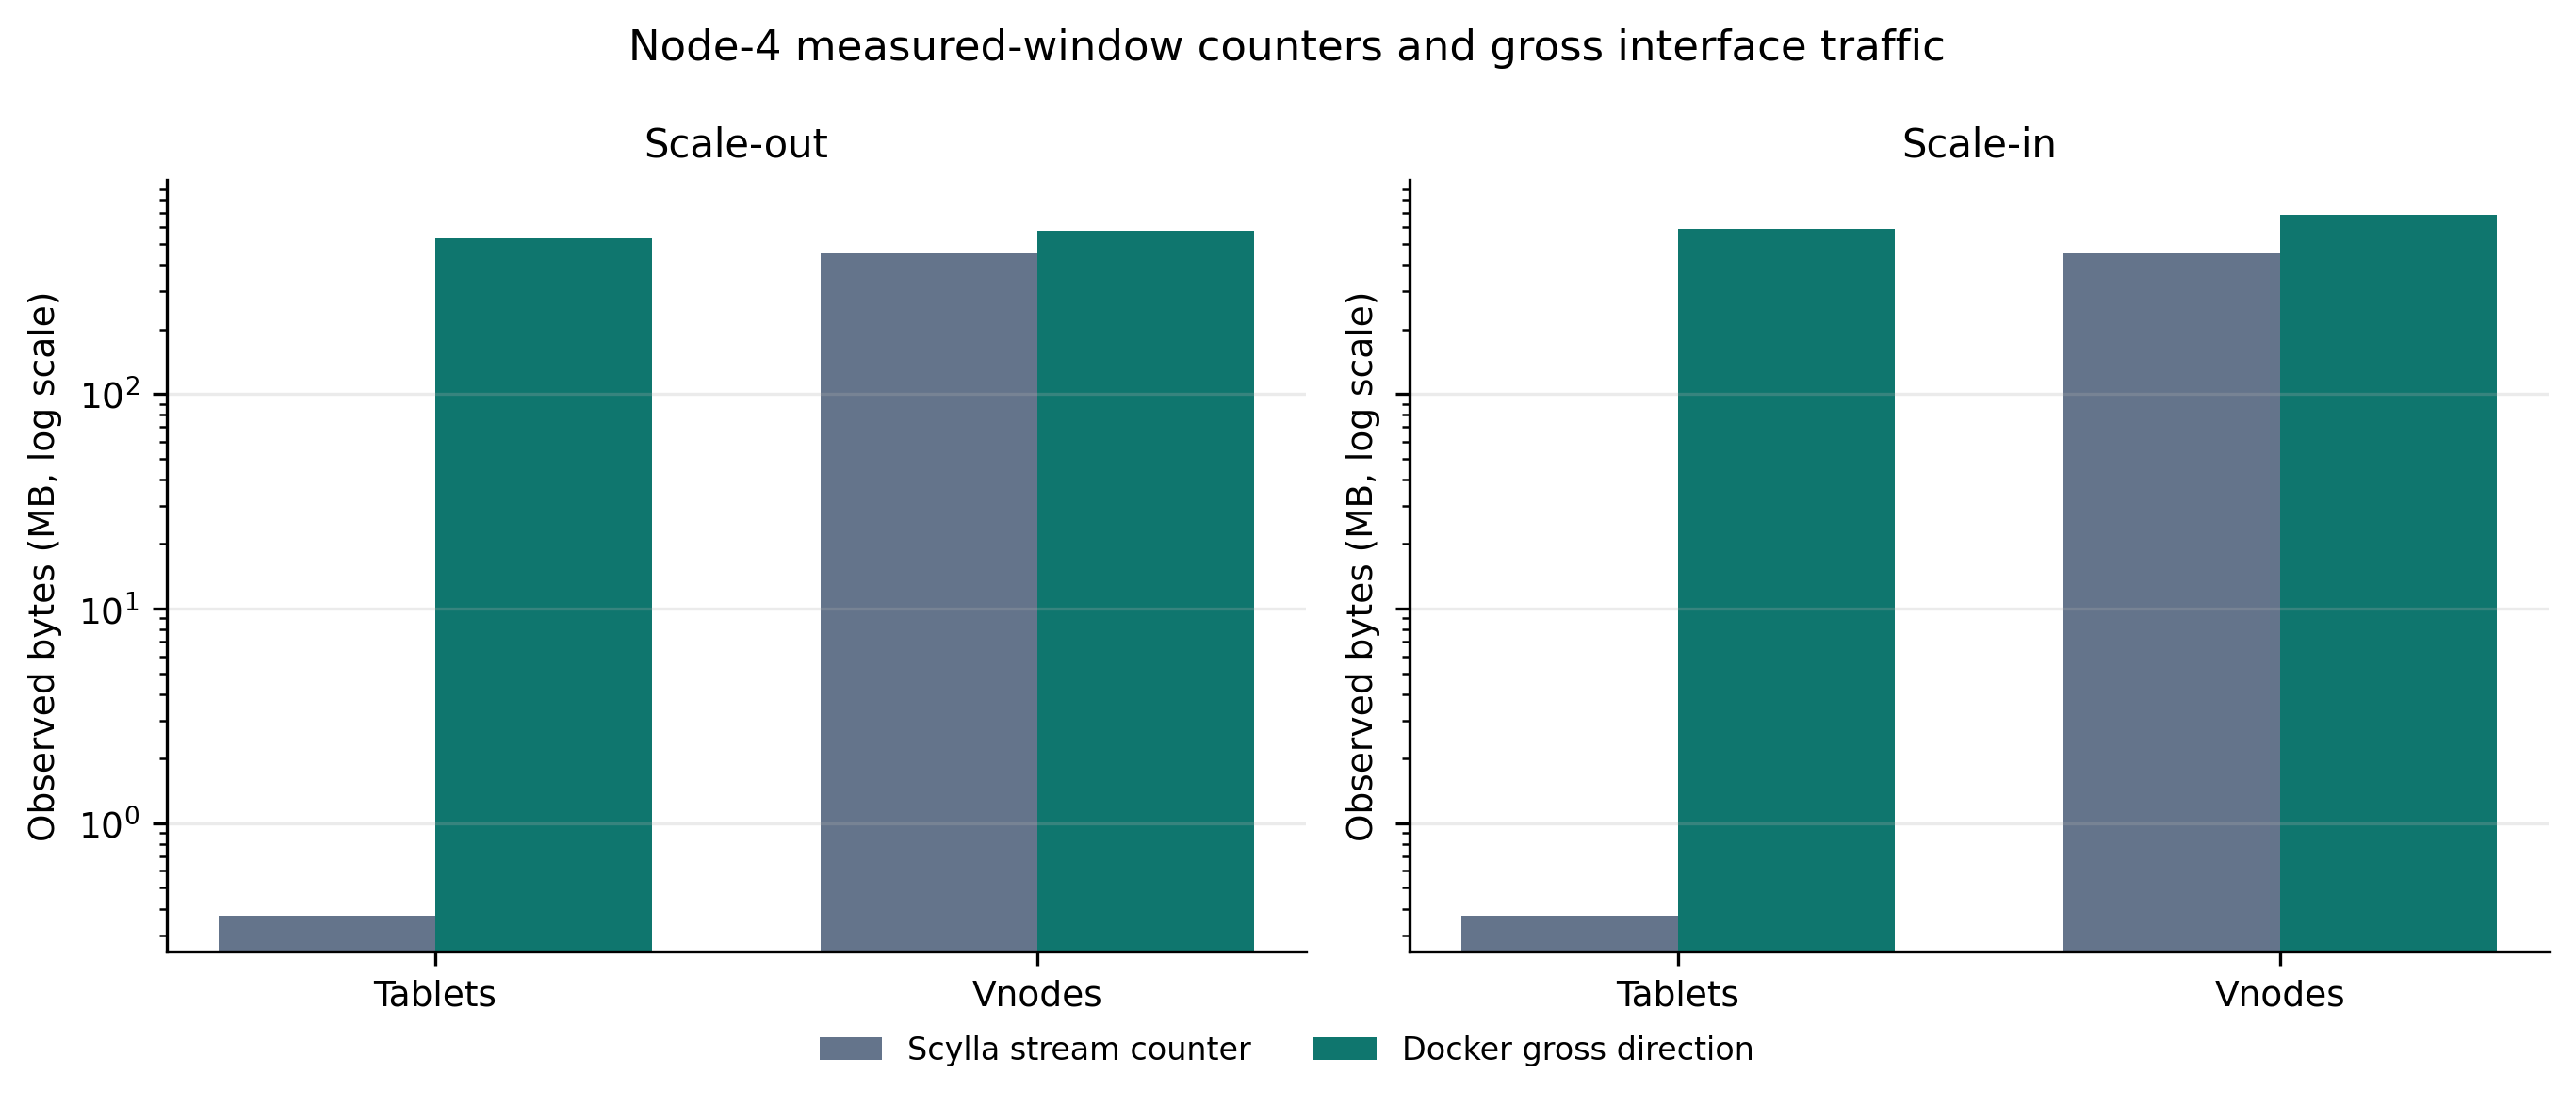
\includegraphics[width=\textwidth,height=.56\textheight,keepaspectratio]{figures/figure_3_movement_observability.png}
\caption{Node-4 directional deltas within measured transition arms: incoming/RX during expansion and outgoing/TX during contraction. Stream counters are 0.369362 MB for tablets and 450.160472 MB for vnodes in each direction. Docker gross deltas are approximately 529 MB for tablets and 578 MB for vnodes during expansion, and 590 MB for tablets and 680 MB for vnodes during contraction. Sampling endpoints and observation durations differ. These measures have different coverage.}\label{fig:figure_3_movement_observability}
\end{figure}

The early vnode receive total, roughly 467 MB, is closer to its stream counter. It still includes unrelated network traffic. Summing interface RX and TX can also count the same transfer twice. Comparing transfer efficiency would require instrumentation that covers the same paths in both treatments.

\newpage

\hypertarget{client-scheduling-immediate-and-delayed-effects}{%
\subsection{Client scheduling: immediate and delayed
effects}\label{client-scheduling-immediate-and-delayed-effects}}

\begin{longtable}[]{@{}lrr@{}}
\caption{Scheduled-start lag, in seconds. The two largest maxima arise
in opposite transition directions. \label{tab:4}}\tabularnewline
\toprule\noalign{}
Treatment / phase & Lag p95 (s) & Maximum (s) \\
\midrule\noalign{}
\endfirsthead
\toprule\noalign{}
Treatment / phase & Lag p95 (s) & Maximum (s) \\
\midrule\noalign{}
\endhead
\bottomrule\noalign{}
\endlastfoot
T / Baseline & 0.190 & 0.334 \\
T / Expansion & 21.876 & 23.070 \\
T / Four-node & 0.283 & 0.496 \\
T / Contraction & 0.114 & 4.425 \\
T / Final three & 0.523 & 0.770 \\
V / Baseline & 0.006 & 0.042 \\
V / Expansion & 1.148 & 8.810 \\
V / Four-node & 0.025 & 0.210 \\
V / Contraction & 21.029 & 23.654 \\
V / Final three & 0.455 & 0.759 \\
\end{longtable}

\begin{figure}[H]
\centering
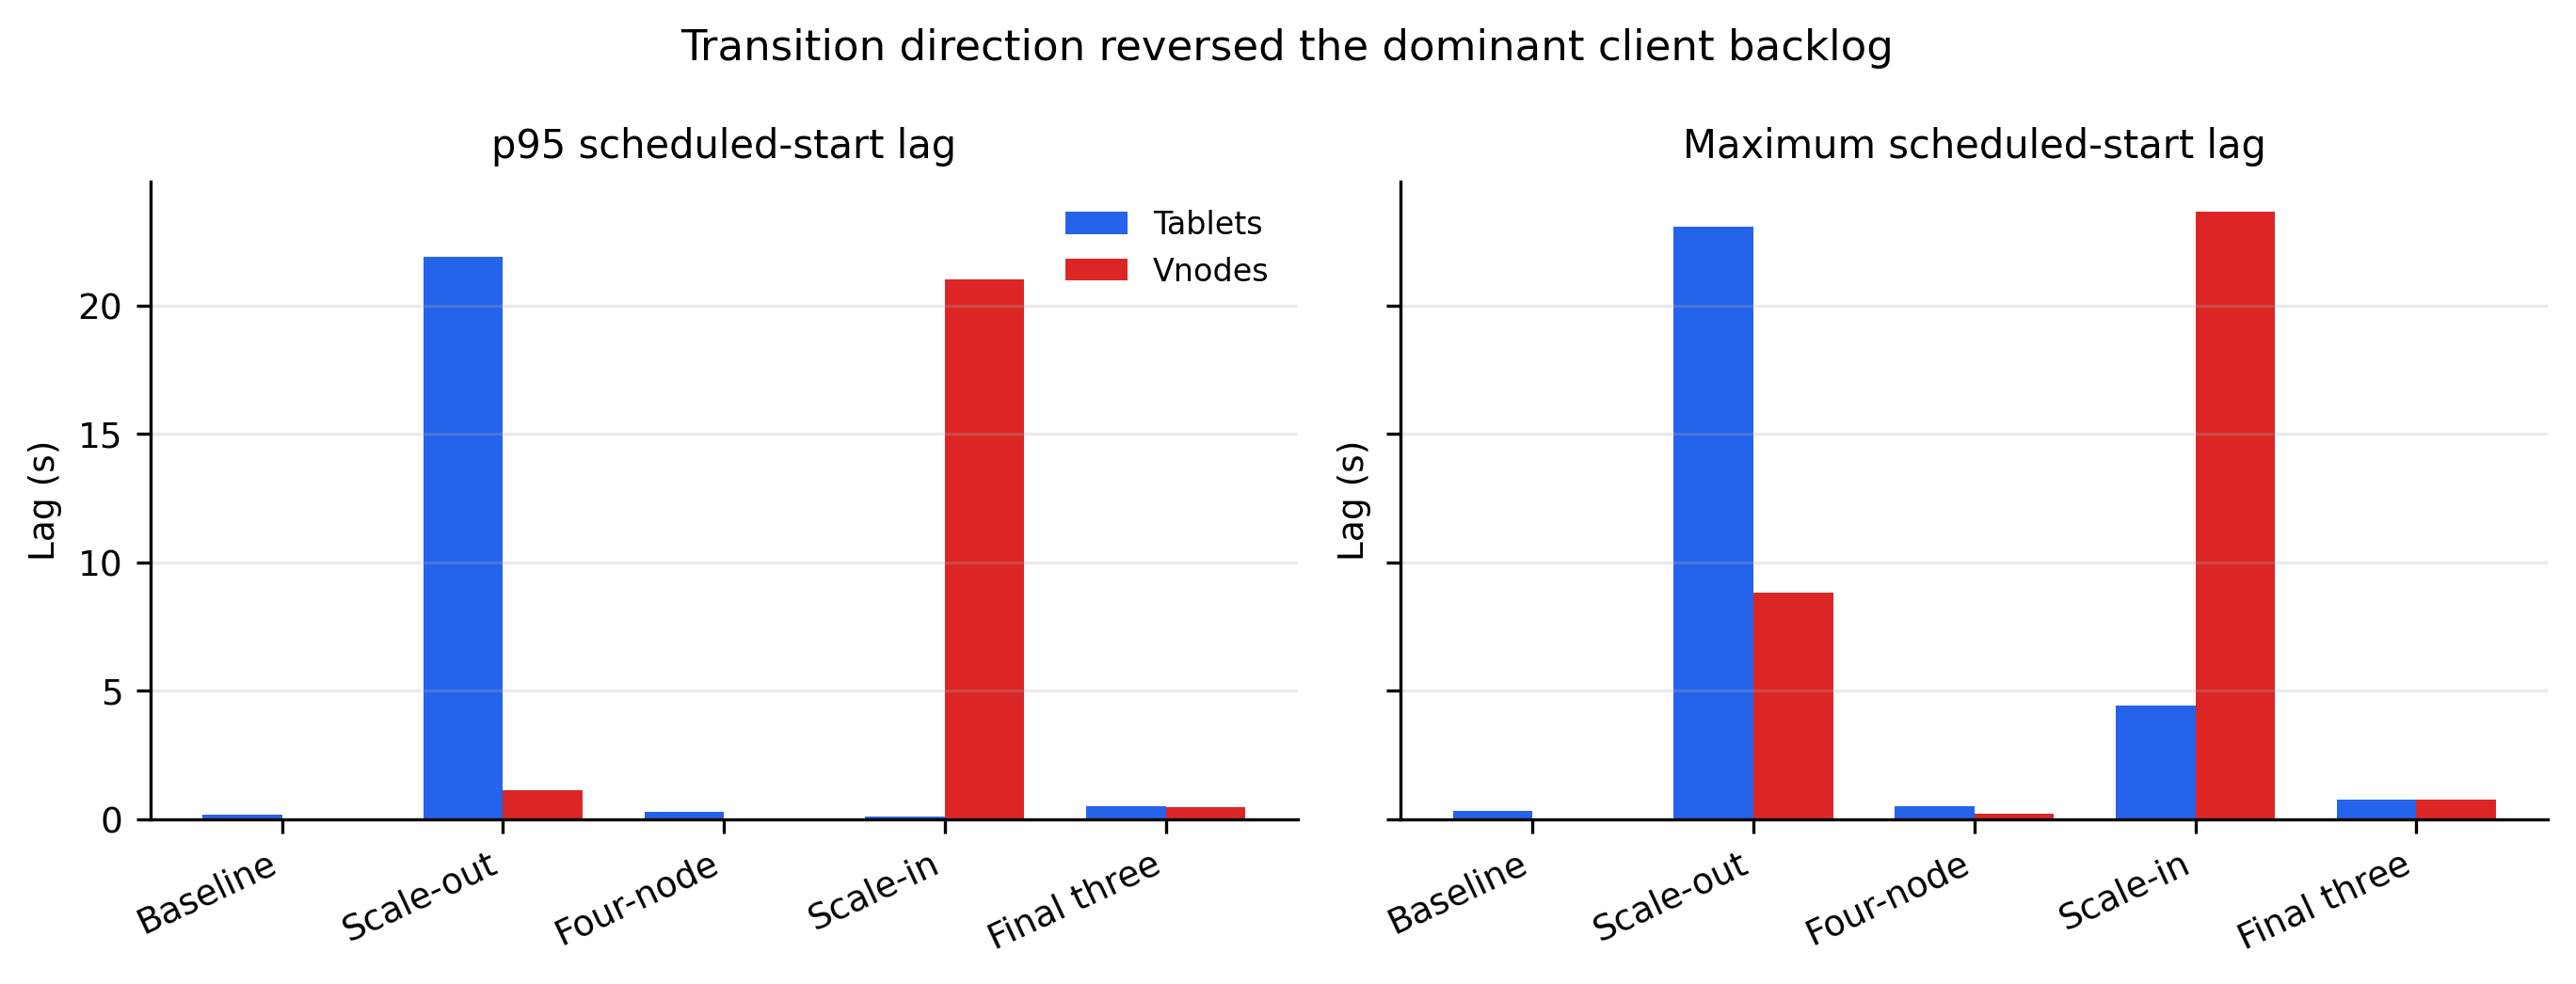
\includegraphics[width=0.8\textwidth,height=0.45\textheight,keepaspectratio]{figures/figure_4_phase_scheduling_lag.png}
\caption{Phase-wide p95 and maximum lag. Mean throughput close to the target obscures temporary backlog followed by catch-up.}\label{fig:figure_4_phase_scheduling_lag}
\end{figure}

\begin{figure}[H]
\centering
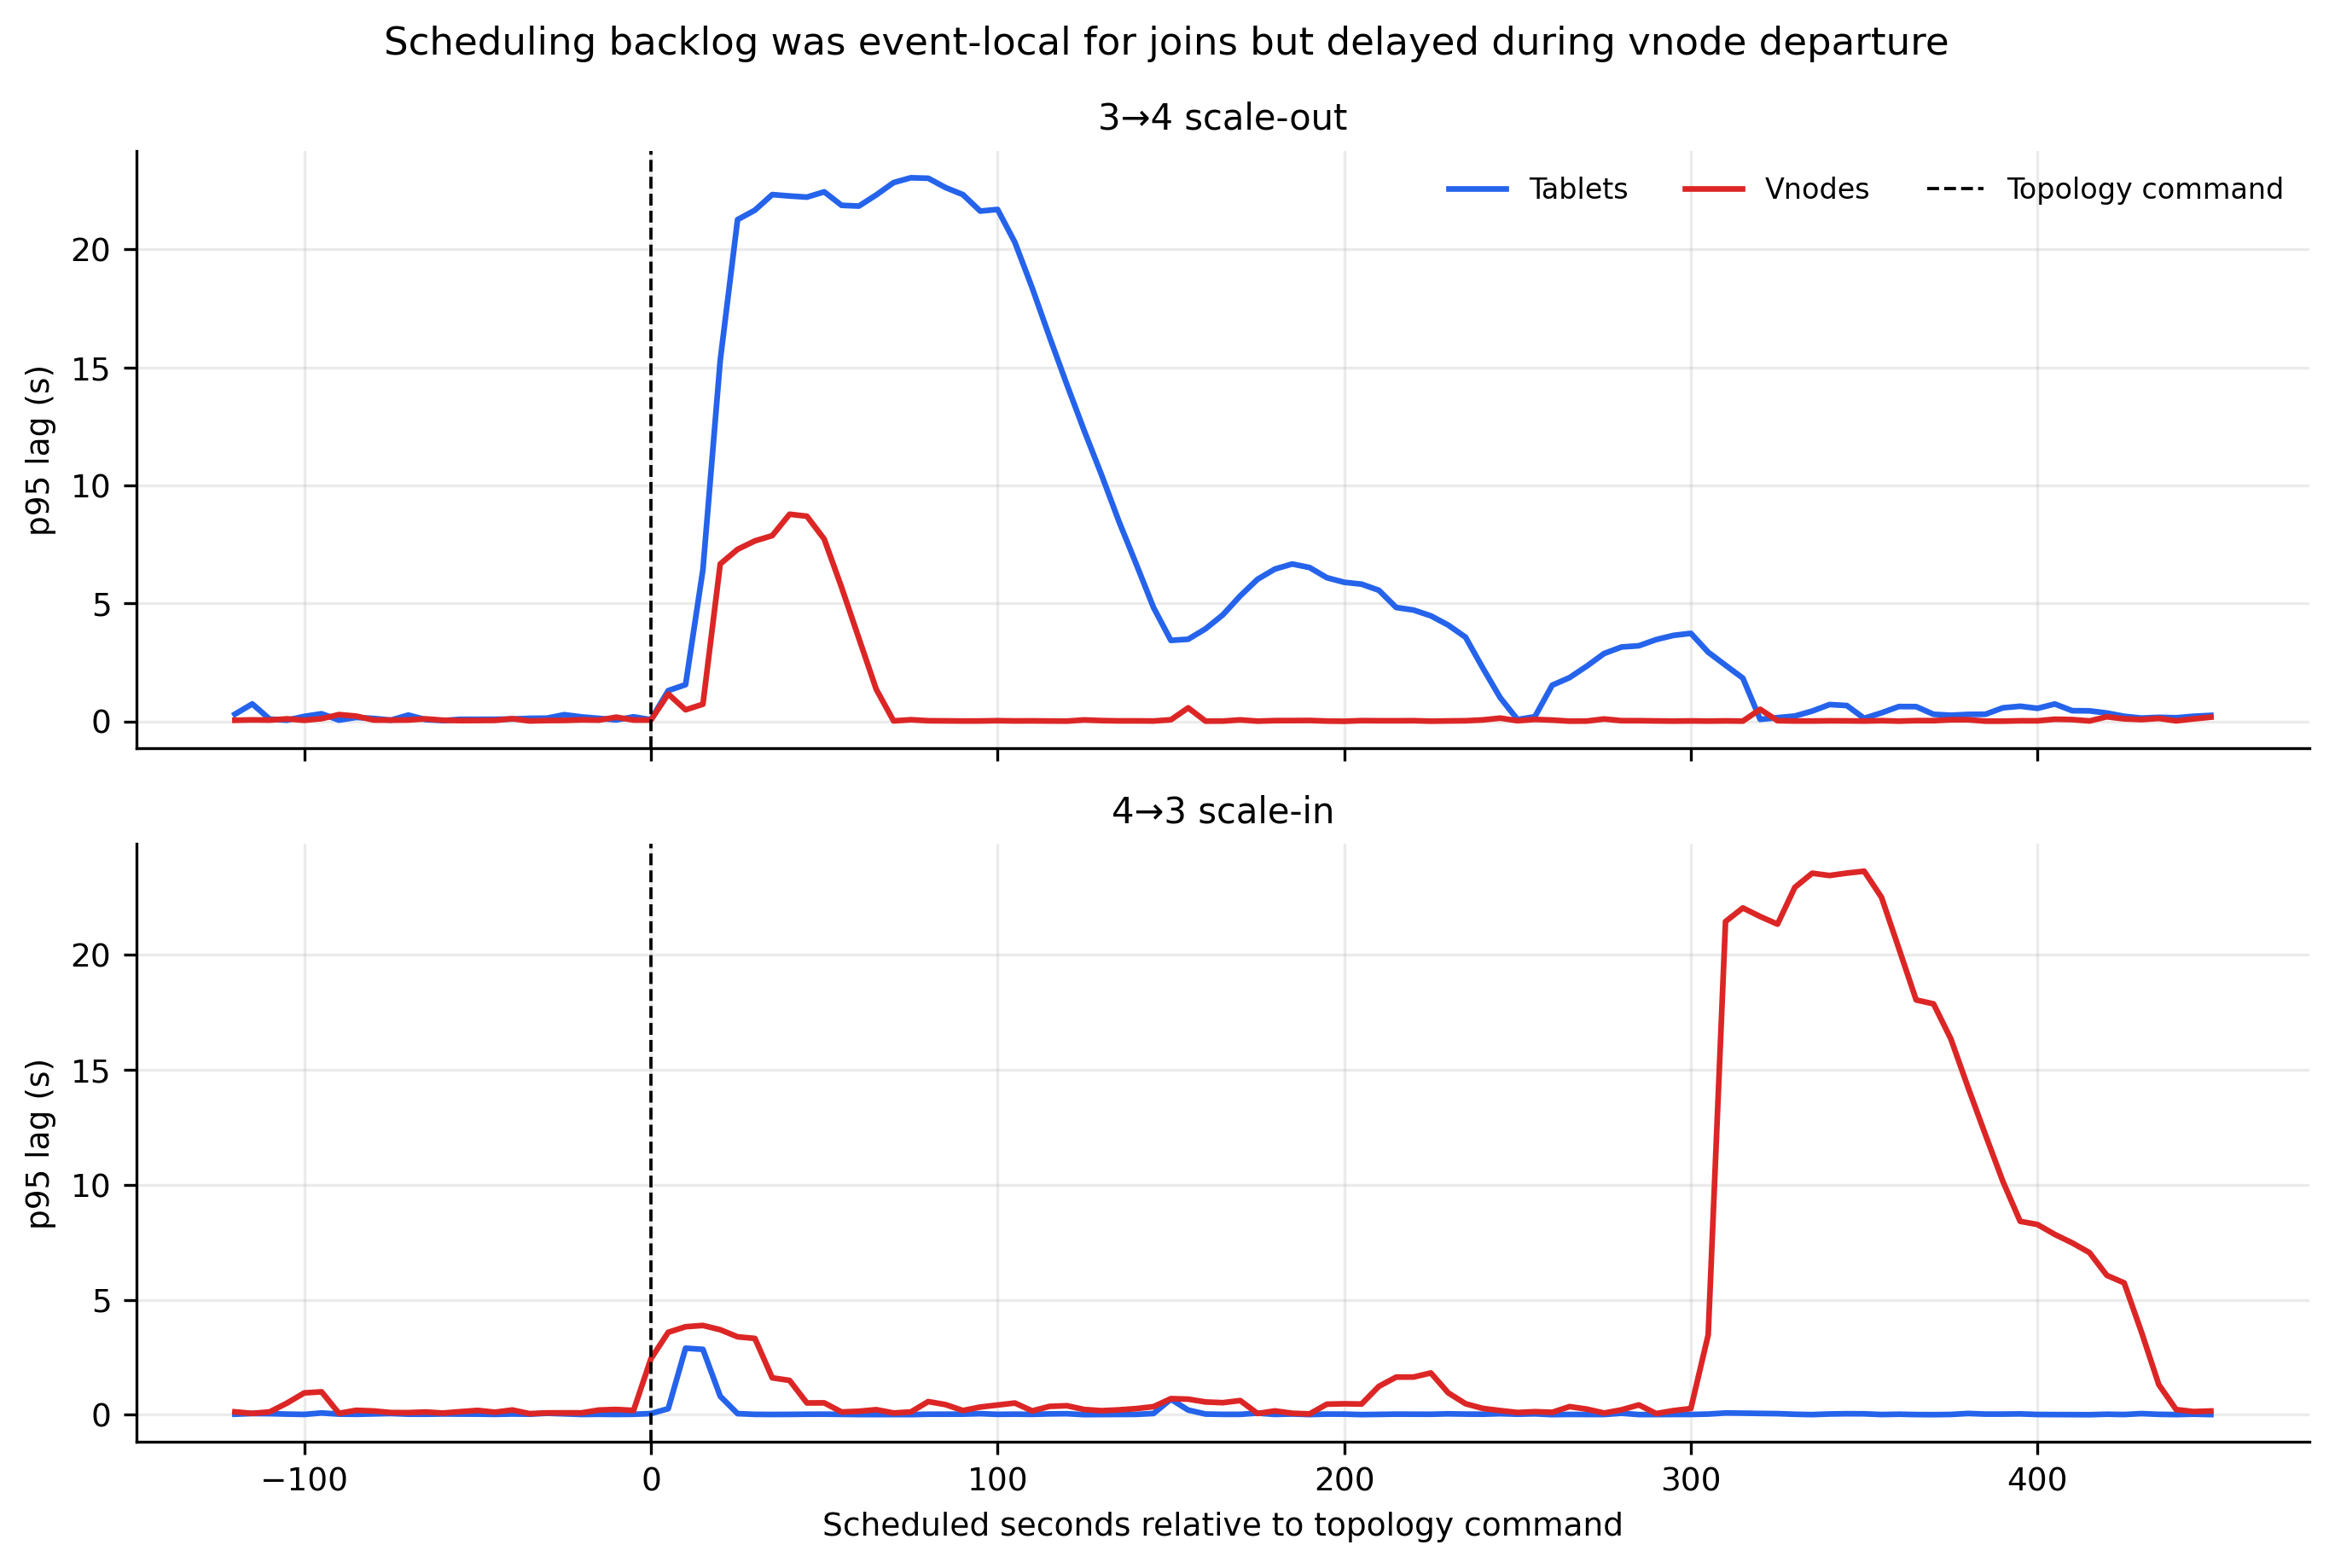
\includegraphics[width=0.8\textwidth,height=0.45\textheight,keepaspectratio]{figures/figure_5_transition_lag_timeline.png}
\caption{Five-second scheduled-time bins around the topology trigger. The view is cropped to -120 through +450 scheduled seconds; smaller later excursions remain in the complete 900-second records. Delayed requests execute later than their scheduled bin.}\label{fig:figure_5_transition_lag_timeline}
\end{figure}

The client trace helps locate where the tablet expansion backlog accumulated. The 15,000 requests scheduled in seconds 90-120 took 29.80 monotonic seconds, including 27.01 seconds inside operations. The next 15,000 took 51.27 seconds. Of that interval, operations consumed 49.18 seconds and the gaps between them consumed 2.08 seconds. Most of the deficit therefore accumulated inside the client operation boundary. Maximum inter-operation gaps were 8.018 and 12.786 ms. Missing tablet server logs prevent a specific server-side diagnosis. Appendix~\ref{measurement-and-evidence-audit} gives the independent timing endpoints and explains the coincidentally similar rounded request-span and topology-onset values.

Vnode expansion also built up backlog, but the maximum was smaller. Its largest five-second scheduled slice took approximately 10.97 seconds to execute, including 10.69 seconds inside operations. Maximum phase lag reached 8.810 seconds, compared with 23.070 for tablets. These traces quantify the temporary service deficit in each run.

Vnode contraction produced two episodes of delay. Lag reached about 3.910 seconds immediately after the command, then recovered. The larger 23.654-second maximum developed approximately five minutes later.

The delayed episode stretches a short scheduled interval across a much longer execution interval. Requests scheduled in seconds 425-435 ran from approximately 15:31:49 to 15:32:20 UTC. Successive groups of 2,500 spent 9.31 and 21.40 seconds inside operations. Node 4 received SIGTERM only at 15:32:34.697. Its later stop therefore cannot explain the initial slowdown.

Receiving data can leave storage maintenance for later. Off-strategy compaction processes SSTables outside the regular compaction strategy; its timing helps explain this second episode. All six surviving-node shards began that work almost simultaneously, approximately 300 seconds after their last logged SSTable receipt. The exact-build source contains a five-minute trigger \cite{r15,r16}. It provides an implementation-consistent explanation for the delay. Appendix~\ref{topology-reconstruction-and-temporal-precision} compares the receipt times, trigger behavior and candidate counts.

Disk activity supports that interpretation. In a surrounding 35.5-second window, nodes 1-3 recorded approximately 2.46 GB of additional block reads and 2.37 GB of writes in total. Node 4's block counters stayed unchanged, and all 16 streaming series stayed flat. The evidence points to delayed local storage work, with no renewed streaming visible in these counters.

The timing still has limits. Compaction-manager messages ended near 15:31:54, while slow operations and later file modification times extended to approximately 15:32:20. The logs cannot explain every millisecond of delay. They establish a temporal association among compaction, shared-host I/O and foreground work. The experiment cannot separate their individual causal contributions.

The impact extends beyond the single worst request. At least five seconds of lag affected 21.488\% of post-event tablet expansion requests and 15.005\% of vnode contraction requests. Appendix~\ref{backlog-exposure} reports exposure at several thresholds. These percentages describe affected requests; they do not measure outage duration.

\newpage

\hypertarget{balance-cleanup-and-storage-history}{%
\subsection{Balance, cleanup and storage
history}\label{balance-cleanup-and-storage-history}}

\begin{longtable}[]{@{}
  >{\raggedright\arraybackslash}p{(\columnwidth - 4\tabcolsep) * \real{0.3333}}
  >{\raggedright\arraybackslash}p{(\columnwidth - 4\tabcolsep) * \real{0.3333}}
  >{\raggedright\arraybackslash}p{(\columnwidth - 4\tabcolsep) * \real{0.3333}}@{}}
\caption{A common logical-placement comparison. RF=2 shares sum to
200\%, apart from rounding. Tablet shares use verified equal-width
ranges; vnode percentages are the ring's effective ownership reports.
\label{tab:5}}\tabularnewline
\toprule\noalign{}
\begin{minipage}[b]{\linewidth}\raggedright
State
\end{minipage} & \begin{minipage}[b]{\linewidth}\raggedright
Tablet token-space shares, N1/N2/N3/N4 (\%)
\end{minipage} & \begin{minipage}[b]{\linewidth}\raggedright
Vnode reported RF=2 shares, N1/N2/N3/N4 (\%)
\end{minipage} \\
\midrule\noalign{}
\endfirsthead
\toprule\noalign{}
\begin{minipage}[b]{\linewidth}\raggedright
State
\end{minipage} & \begin{minipage}[b]{\linewidth}\raggedright
Tablet token-space shares, N1/N2/N3/N4 (\%)
\end{minipage} & \begin{minipage}[b]{\linewidth}\raggedright
Vnode reported RF=2 shares, N1/N2/N3/N4 (\%)
\end{minipage} \\
\midrule\noalign{}
\endhead
\bottomrule\noalign{}
\endlastfoot
Initial three & 65.625 / 68.750 / 65.625 / - & 65.48 / 63.78 / 70.74 /
- \\
Four-node & 50 / 50 / 50 / 50 & 50.86 / 47.08 / 53.40 / 48.67 \\
Final three & 65.625 / 68.750 / 65.625 / - & 65.48 / 63.78 / 70.74 /
- \\
\end{longtable}

At the four-node endpoint, tablets distributed both assignments and reported bytes evenly. Each node held exactly 32 replicas. Reported bytes were 400,686,101; 401,861,023; 400,458,341; and 399,372,064. Their coefficient of variation was approximately 0.22\%. The maximum-minus-minimum difference was 0.62\% of the mean. Logical token-space variation was zero. Vnode four-node ownership had a coefficient of variation of approximately 4.753\%. These measurements characterize this dataset, token realization and observed cluster.

\begin{figure}[H]
\centering
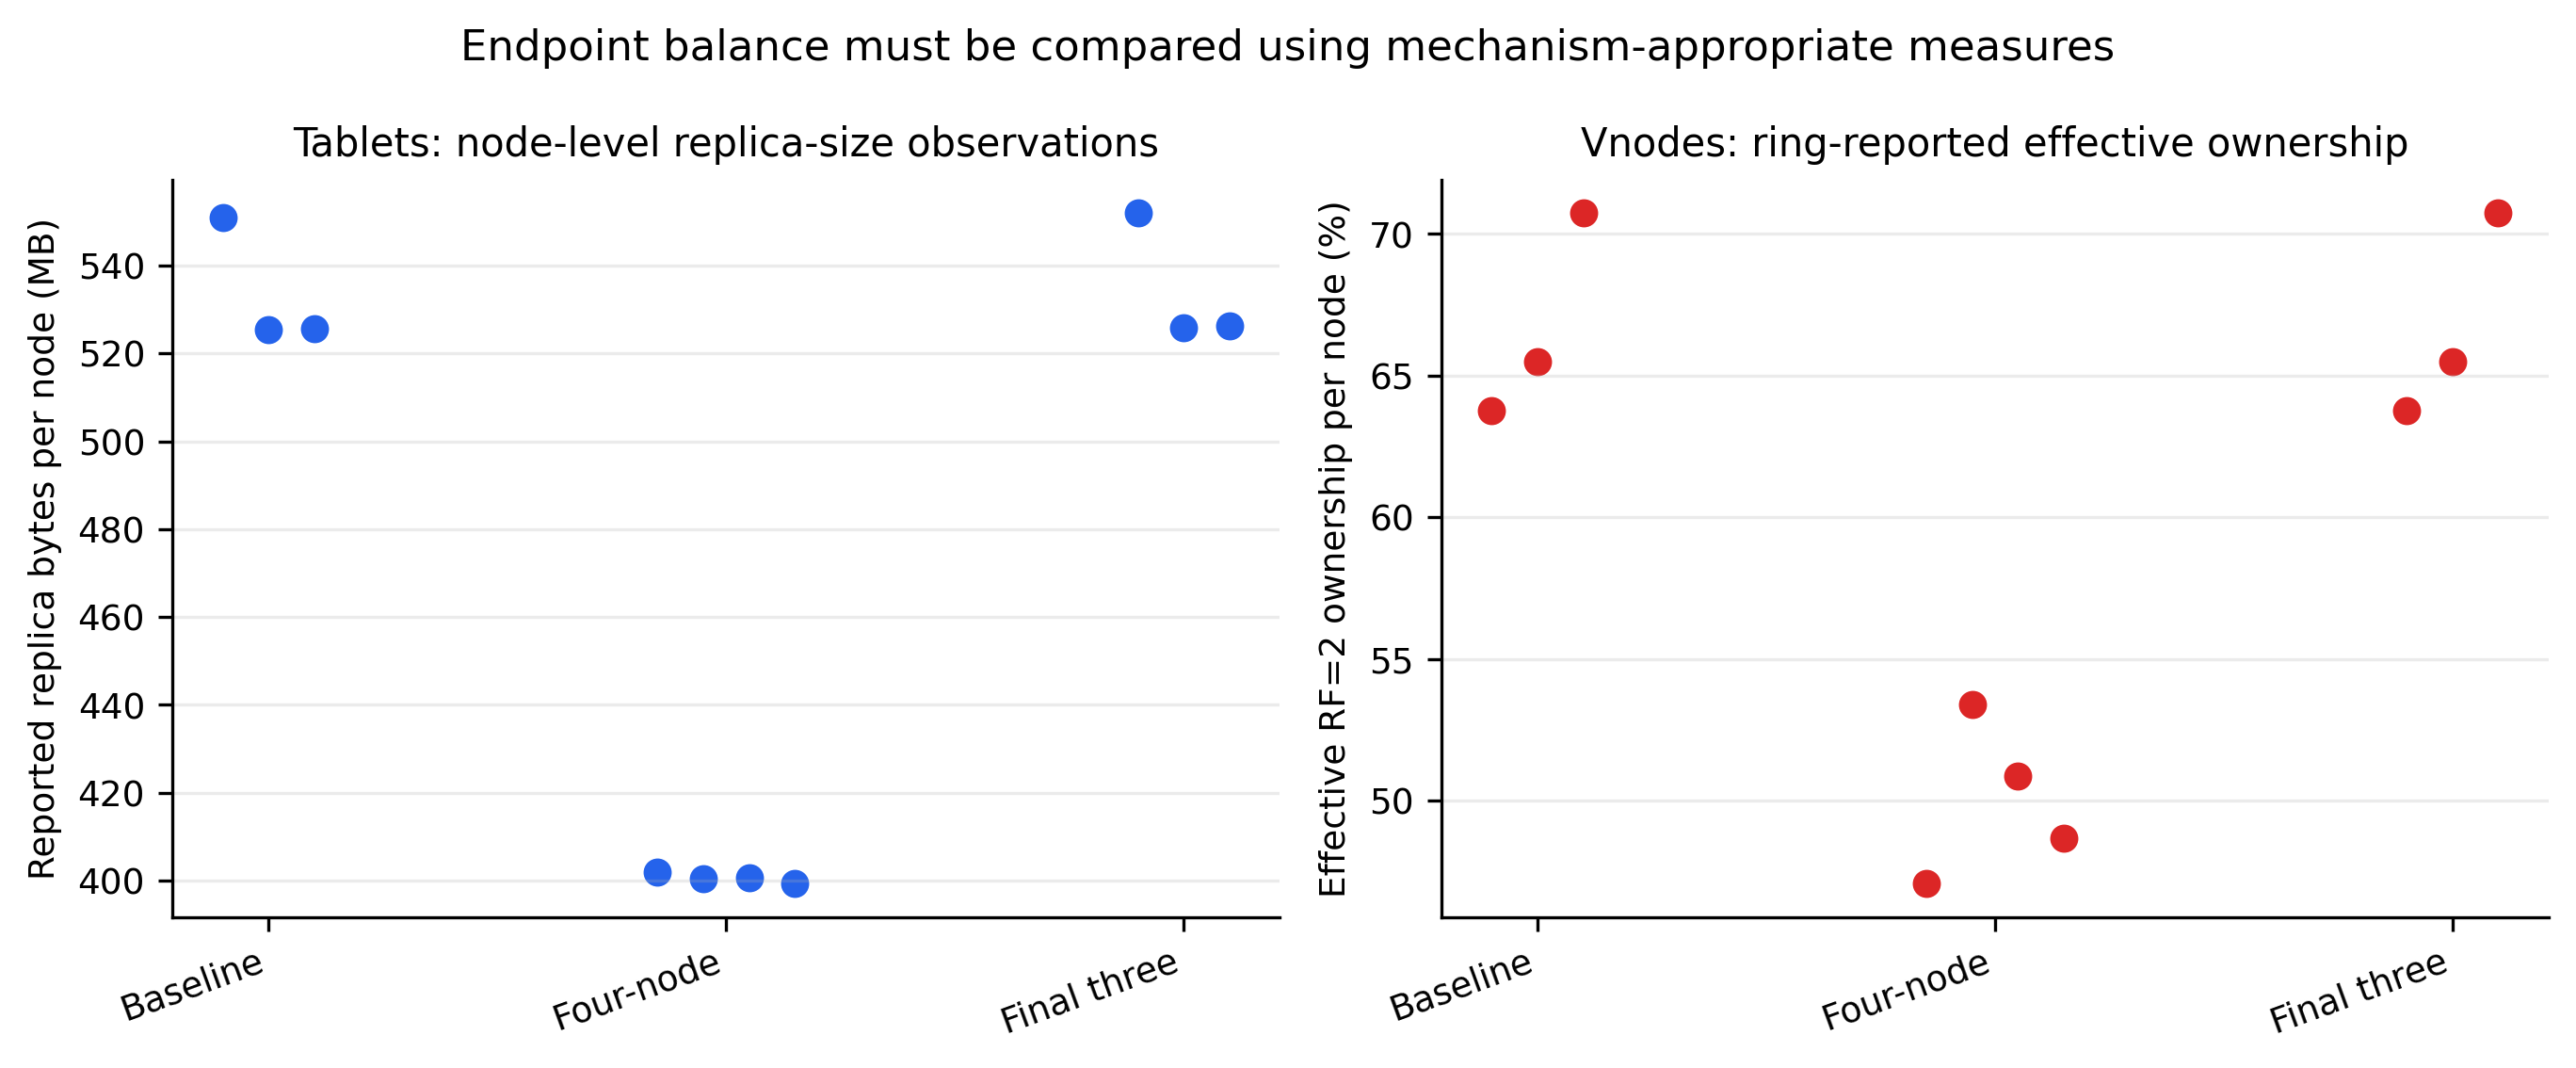
\includegraphics[width=\textwidth,height=.56\textheight,keepaspectratio]{figures/figure_6_endpoint_balance.png}
\caption{Tablet reported replica-size bytes and vnode effective ownership at lifecycle endpoints. The panels deliberately retain their respective units; Table~\ref{tab:5} supplies the direct token-space comparison.}\label{fig:figure_6_endpoint_balance}
\end{figure}

Placement changes do not necessarily reclaim obsolete files immediately. After vnode expansion, the original nodes initially retained their previous live-byte totals. Cleanup removes data for ranges a node no longer owns \cite{r13,r14}. The serial cleanup commands took 4.398, 2.939 and 2.882 seconds, or 10.219 seconds combined. The surrounding wall interval lasted approximately 180.780 seconds. It included 170.561 seconds of checks/operator gaps, which are separate from cleanup service time.

After cleanup, the original nodes reported 459,724,966; 417,238,653; and 481,774,985 live bytes. The total fell by 244,740,998 bytes. Cleanup and flushing both changed storage state, so obsolete-data removal cannot explain the entire reduction on its own. The original nodes had zero memtable bytes, while node 4 still held 54,148,158. The subsequent four-node phases therefore began with different cache and memtable histories.

At the final vnode checkpoint, live bytes were 525,841,391; 523,193,434; and 633,114,947. The nodes held 2/4/6 SSTables and reported partition estimates of 491,495/488,925/592,081. Their byte spread was 19.60\% of the mean. Tablets ended with 21/22/21 replicas and 526,231,881/551,974,438/525,773,936 reported bytes, a spread of 4.90\%.

The vnode totals raised a further question: how much of the apparent imbalance came from overlapping files? Disk totals combine ownership with file overlap and maintenance history. Table~\ref{tab:5} isolates the logical shares; the next audit examines the files.

\hypertarget{resolving-the-vnode-final-partition-count-excess}{%
\subsection{Resolving the vnode final partition-count
excess}\label{resolving-the-vnode-final-partition-count-excess}}

The final vnode estimates suggested more replicas than RF=2 required. They summed to 1,572,501, exceeding the nominal 1,500,000 node-key pairs by 72,501. A key can occur in several SSTables on one node, so counting entries alone cannot distinguish local overlap from extra distinct replicas.

We tested that distinction directly. We mounted the preserved volumes read-only and used the matching offline SSTable tools \cite{r23}. The selected 12 files matched the pre-shutdown 2/4/6-file checkpoint. We excluded two later shutdown-time files per node. The audit therefore covers that retained file set, rather than every file eventually present in the volumes.

Before comparing nodes, we checked the extraction itself. In all 12 files, extracted partition-key counts matched the per-file \texttt{rows\_count} metadata. Every ID fell within the dataset range. No file contained repeated extracted IDs.

\begin{longtable}[]{@{}
  >{\raggedright\arraybackslash}p{(\columnwidth - 6\tabcolsep) * \real{0.2000}}
  >{\raggedleft\arraybackslash}p{(\columnwidth - 6\tabcolsep) * \real{0.2667}}
  >{\raggedleft\arraybackslash}p{(\columnwidth - 6\tabcolsep) * \real{0.2667}}
  >{\raggedleft\arraybackslash}p{(\columnwidth - 6\tabcolsep) * \real{0.2667}}@{}}
\caption{Exact key accounting for the selected final-checkpoint
SSTables. The sum of distinct local IDs counts replicas across nodes,
not globally distinct keys. \label{tab:6}}\tabularnewline
\toprule\noalign{}
\begin{minipage}[b]{\linewidth}\raggedright
Node
\end{minipage} & \begin{minipage}[b]{\linewidth}\raggedleft
SSTable entries
\end{minipage} & \begin{minipage}[b]{\linewidth}\raggedleft
Distinct local IDs
\end{minipage} & \begin{minipage}[b]{\linewidth}\raggedleft
Repeated entries across local files
\end{minipage} \\
\midrule\noalign{}
\endfirsthead
\toprule\noalign{}
\begin{minipage}[b]{\linewidth}\raggedright
Node
\end{minipage} & \begin{minipage}[b]{\linewidth}\raggedleft
SSTable entries
\end{minipage} & \begin{minipage}[b]{\linewidth}\raggedleft
Distinct local IDs
\end{minipage} & \begin{minipage}[b]{\linewidth}\raggedleft
Repeated entries across local files
\end{minipage} \\
\midrule\noalign{}
\endhead
\bottomrule\noalign{}
\endlastfoot
1 & 491,495 & 491,495 & 0 \\
2 & 488,925 & 477,873 & 11,052 \\
3 & 592,081 & 530,632 & 61,449 \\
Total & 1,572,501 & 1,500,000 node-ID pairs & 72,501 \\
\end{longtable}

Deduplication resolved the apparent excess completely. The union contained exactly 750,000 IDs, and every ID appeared on exactly two nodes. None appeared on one or three. Repeated keys across local SSTables accounted for all 72,501 excess entries, leaving no unexplained residual in the selected file set. The distinct local counts also matched the initial post-load counts.

This result establishes local file overlap within the selected files. The audit did not reconstruct memtables, latest values, timestamps or an atomic historical snapshot. A separate excess of 135,784 in the four-node post-cleanup estimate remains unallocated. We lack that historical file set in the same form. The final-checkpoint result cannot establish its earlier composition.

\newpage

\hypertarget{discussion}{%
\section{Discussion}\label{discussion}}

\hypertarget{the-mechanisms-expose-different-notions-of-completion}{%
\subsection{The mechanisms expose different notions of
completion}\label{the-mechanisms-expose-different-notions-of-completion}}

Returning to three members did not erase the lifecycle's history. Tablets migrated replicas, aligned shards, split and merged ranges, then redistributed again. Their final boundary count and aggregate replica counts matched the initial values, while individual assignments changed. Vnodes restored their original token-owner signature, but streaming and overlapping SSTables left a different local file history. Logical placement and physical storage therefore describe complementary outcomes.

The delayed vnode episode makes the operational consequence clear. An unchanged ring and idle streaming counters satisfy the defined quiescence condition even when deferred storage work remains. Client recovery adds another timescale. Once operations become faster, the serial client can temporarily exceed the target rate and clear its backlog. A near-target phase average can therefore hide substantial disruption within the phase.

\hypertarget{multiple-outcomes-and-scope}{%
\subsection{Multiple outcomes and
scope}\label{multiple-outcomes-and-scope}}

The comparison yields several concrete results. Tablets reached equal four-node token-space shares without manual post-join cleanup in this lifecycle. Vnodes reached the placement-and-counter milestone earlier. The smaller client backlog belonged to a different treatment in each transition direction. Offline extraction then explained the final physical-count anomaly. Together, these findings show why engineers need several endpoints to evaluate elasticity.

\textbf{Scope and limitations.} The comparison covers one lifecycle per treatment in a fixed order. Unequal baselines, inter-phase gaps and vnode-only cleanup limit causal inference. All processes share CPU, NVMe storage, filesystem cache and host memory. The 161-MiB Windows observation alone cannot establish paging. I did not record effective VM vCPU limits or exact configured memory.

The evidence also differs between treatments. Vnode logs support the deferred-compaction explanation; missing tablet logs leave its expansion slowdown without a server-side diagnosis. Source inspection identifies mechanisms consistent with the observations. It cannot establish historical runtime choices where settings are missing. Sampled quiescence covers only recorded metadata and counters, and the study did not calibrate independent collector clock offsets. These constraints support a descriptive single-host case study. Treatment-level repeatability and production generalization remain open.

\hypertarget{future-work}{%
\subsection{Future work}\label{future-work}}

Repeated, counterbalanced runs on multiple hosts could estimate variability and separate treatment effects from execution history. Recording effective runtime configuration and retaining server logs for both treatments would strengthen mechanism attribution. Controlled maintenance could isolate deferred storage effects. Instrumentation covering the same transfer paths could support a direct comparison of migration bytes. Further experiments could vary workload concurrency, replication and dataset size.

\newpage

\hypertarget{conclusion}{%
\section{Conclusion}\label{conclusion}}

This study compared how tablets and vnodes expand and contract under a matched workload. Both ScyllaDB lifecycles completed 1.08 million requests without reported workload failures and retained 750,000 logical keys. Their behavior differed in placement balance, redistribution, maintenance and client recovery. The central finding is that these processes finish at different times. An early topology milestone can precede a substantial later backlog.

Tablets achieved equal four-node replica counts and token-space shares, with closely balanced reported bytes. Vnodes retained unequal replicated shares despite equal token counts. Tablets returned from 64 to their original 32 boundaries, but 11 ranges ended on different host sets. Vnodes restored their original token ownership while retaining a different local file history. Aggregate endpoints therefore concealed distinct paths through the lifecycle.

The tablet metadata explains those paths in detail. Pending assignments reconciled split inheritance and merge alignment. An intra-node shard migration aligned a merge pair, and a further inter-node migration followed the merge. These observations show why a stable tablet count alone cannot establish stable placement.

The client comparison also changed with transition direction. Maximum expansion lag was 23.070 seconds for tablets and 8.810 seconds for vnodes. Maximum contraction lag was 4.425 and 23.654 seconds, respectively. Vnodes reached placement-and-counter quiescence earlier in both directions. Yet their largest contraction backlog arrived approximately five minutes after streaming reception, alongside synchronized deferred compaction and substantial disk activity. The source's five-minute trigger provides a mechanism consistent with that timing. The evidence associates these events without assigning the entire slowdown to compaction alone.

The storage audit resolved another misleading signal. Exact offline key extraction accounted for all 72,501 excess final vnode SSTable entries as overlap across files on the same node. Within the selected pre-shutdown files, all 750,000 keys appeared on exactly two nodes. Summed file entries had overstated distinct replicas. The earlier four-node excess remains outside that exact accounting because its historical file set is unavailable.

Monitoring coverage proved equally important. The collected stream counters omit the full tablet file-transfer path, so their totals cannot support a direct comparison of total movement. The missing tablet size reports also followed a specific pattern: outgoing replicas disappeared from size observations during transitions, and every destination appeared with a positive size in the next snapshot. Combining independent evidence explained these apparent inconsistencies.

The contribution is a detailed comparative account of how the two mechanisms behaved and why individual metrics could mislead. The study connects placement changes, client backlog, deferred maintenance and physical key accounting. Unequal starting performance, shared resources, asymmetric logs and one lifecycle per treatment keep the performance comparison descriptive. In particular, the tablet expansion slowdown still lacks a specific server-side diagnosis. Repeated studies can test how consistently these differences recur. For the observed lifecycles, the practical lesson is clear: evaluate placement convergence, storage completion and client recovery together.

\hypertarget{data-and-code-availability}{%
\section{Data and code
availability}\label{data-and-code-availability}}

The project repository provides the workload, monitoring and analysis scripts, Docker definitions, derived summaries and figure sources \cite{r35}. I retain approximately 949~MiB of raw observations separately and will provide them on request through the \href{https://github.com/GiorgiGogsadze/Scylla-Research/issues}{repository issue tracker}. The analysis manifest hashes the derived outputs only. Appendix~\ref{reproducibility-and-preserved-evidence} describes the preserved evidence and the repository revision inspected.

\newpage

\appendix

\hypertarget{measurement-and-evidence-audit}{%
\section{Measurement and evidence
audit}\label{measurement-and-evidence-audit}}

\hypertarget{clocks-and-client-accounting}{%
\subsection{Clocks and client
accounting}\label{clocks-and-client-accounting}}

The clock audit separates wall-clock artifacts from client backlog. Across all ten measured request files, indices were valid and monotonic starts increased strictly. No inter-operation gap fell below -0.01 ms. UTC starts nevertheless stepped backward 38 times in tablet files and 50 times in vnode files. Another 83 UTC operation spans were negative. The largest UTC backstep was 2.157 ms. The largest adjacent change in UTC-versus-monotonic drift was 5.354 ms.

UTC spans were 9.450-16.834 ms shorter than monotonic spans in 120-second phases. The difference was 71.824-92.904 ms in 900-second phases. These small wall-clock effects cannot explain the multi-second monotonic scheduling backlogs.

Different timing boundaries also explain apparently inconsistent throughput figures. The workload's completion banner includes final CSV/state persistence but excludes some setup and teardown work. The vnode final warmup banner reported 485.92/s. Its first-request-to-last-completion span was 30.204 seconds, or approximately 496.61/s. We retain UTC-derived request-span rates as descriptive summaries. Monotonic fields remain the basis for lag and operation duration.

Two intervals happen to round to 51.265 seconds. They have different endpoints and use different clocks. The tablet topology interval starts with the join command at 17:41:59.0830105 UTC and ends with the first accepted observation at 17:42:50.347804 UTC. It lasts 51.2647935 seconds, rounded to 51.265.

The raw-request audit instead records 51.265243 monotonic seconds for the 15,000 requests scheduled in seconds 120-150. Their UTC endpoints are 17:41:58.859705 and 17:42:50.120515, giving 51.260810 seconds. The archived five-second bins corroborate those endpoints. The near equality is coincidental. Monotonic accounting divides this request window into 49.182314 seconds inside operations and 2.082929 between them. For the preceding window, those components are 27.012917 and 2.785911 seconds.

\hypertarget{coverage-and-parser-corrections}{%
\subsection{Coverage and parser
corrections}\label{coverage-and-parser-corrections}}

\begin{longtable}[]{@{}
  >{\raggedright\arraybackslash}p{(\columnwidth - 4\tabcolsep) * \real{0.3333}}
  >{\raggedright\arraybackslash}p{(\columnwidth - 4\tabcolsep) * \real{0.3333}}
  >{\raggedright\arraybackslash}p{(\columnwidth - 4\tabcolsep) * \real{0.3333}}@{}}
\caption{Saved observations within measured request intervals. Each
collector also bracketed the interval. Sampling counts need not equal
duration because commands take time and cadence varies.
\label{tab:A1}}\tabularnewline
\toprule\noalign{}
\begin{minipage}[b]{\linewidth}\raggedright
Phase
\end{minipage} & \begin{minipage}[b]{\linewidth}\raggedright
Tablet snapshots / stream / Docker samples
\end{minipage} & \begin{minipage}[b]{\linewidth}\raggedright
Vnode ring / stream / Docker samples
\end{minipage} \\
\midrule\noalign{}
\endfirsthead
\toprule\noalign{}
\begin{minipage}[b]{\linewidth}\raggedright
Phase
\end{minipage} & \begin{minipage}[b]{\linewidth}\raggedright
Tablet snapshots / stream / Docker samples
\end{minipage} & \begin{minipage}[b]{\linewidth}\raggedright
Vnode ring / stream / Docker samples
\end{minipage} \\
\midrule\noalign{}
\endhead
\bottomrule\noalign{}
\endlastfoot
Baseline & 115 / 120 / 35 & 59 / 120 / 36 \\
Expansion & 857 / 897 / 261 & 436 / 896 / 266 \\
Four-node & 114 / 120 / 35 & 58 / 120 / 36 \\
Contraction & 863 / 900 / 270 & 435 / 893 / 259 \\
Final three & 114 / 120 / 35 & 58 / 120 / 35 \\
\end{longtable}

Nine tablet size snapshots were incomplete: seven during expansion and two during contraction. They contained 12 missing-replica reports. Ten occurred at \texttt{end\_migration}, and two occurred at \texttt{cleanup}. Every missing host was an outgoing replica, and the token sets still matched.

In all 12 cases, the same snapshot lacked a destination size. The immediately following snapshot showed a positive destination size, current placement and a cleared transition, 1.021-1.087 seconds later. Three cases crossed the split, so the next size describes a child range. We excluded incomplete samples from byte-balance endpoints. A missing size observation does not establish a zero-size or unavailable replica.

The parsers handle the formats present in the saved evidence. Seven ring snapshots report node-4 load as \texttt{?}, while retaining all 256 of its rows. The ring parser accepts that form alongside numeric sizes. All 5,358 raw ring-file hashes and address counts passed validation. Docker size parsing accepts scientific notation such as \texttt{1e+03MB}. The SSTable key extractor handles records that cross input-chunk boundaries. Its counts matched metadata in all 12 selected files, including the 5,555-key test case.

Nodes 1-3 contributed 135,370,928, 153,890,512 and 160,899,032 bytes to the vnode expansion counters. Contraction recorded the same amounts in reverse. Tablet expansion contributions were 46,152, 184,898 and 138,312 bytes. None of the audited series decreased. Initial visibility remains a limit: node 4 first supplied metrics approximately 7.587 seconds after tablet join initiation and 6.805 seconds after vnode initiation.

\hypertarget{acquisition-and-operational-qualifications}{%
\subsection{Acquisition and operational
qualifications}\label{acquisition-and-operational-qualifications}}

The complete tablet record contains 6,947 snapshot-index entries, 7,160 complete streaming samples and 7,194 Docker rows. The vnode record contains 5,358 indexed ring samples, 10,976 complete streaming samples and 10,794 Docker rows. Event logs contain 16 tablet records and 22 vnode records. These include five phase starts and ends per treatment, plus vnode cleanup events.

Health checks reported zero pending tasks and no outgoing streams at the stated checkpoints. Container inspections found no restarts or OOM flags at inspection time. The Docker CSV did not record those fields continuously.

Retained vnode logs include startup, cleanup and departure warnings. Node-1 cleanup produced reclaim warnings of 44, 76 and 124 ms outside the measured expansion arm. Transient gossip/raft messages accompanied membership changes. SIGTERM/abort messages accompanied the stop of node 4. This timing documents the warnings without establishing that every warning was harmless.

After decommissioning, node 4's process remained observable even though it had left the ring. Resource and streaming collectors therefore continued to report four processes. Confirmed process absence came about 149.962 seconds after tablet decommission initiation and 356.808 seconds after vnode initiation. Later observations verified unchanged three-node placement.

Post-decommission statistics were partial. Tablets returned an HTTP 500 closed snapshot-gate error from \texttt{tablestats}. Vnodes returned exit code 4 with partial output. Neither failed call establishes a zero-partition count.

The gaps from one phase-end marker to the next phase-start marker were approximately 1,137/761/1,456/553 seconds for tablets. Vnode gaps were 3,574/1,541/1,552/1,290 seconds. These intervals include checks and warmups as well as idle time. Repeating the vnode expansion warmup changed its rate from 470.16/s to 498.52/s and its maximum lag from 1.771 seconds to 0.258 seconds. Both warmups remain outside the measured replicates.

Summed observed container-memory peaks were approximately 6.12/6.20 GiB for tablet/vnode expansion and 6.32/6.42 GiB for contraction. Maximum sampled single-container CPU percentages were 189.60/86.76 during expansion and 142.75/144.50 during contraction. Docker CPU percentages can exceed 100\% for a multi-core process. These samples locate activity in time but do not establish its cause.

\newpage

\hypertarget{topology-reconstruction-and-temporal-precision}{%
\section{Topology reconstruction and temporal
precision}\label{topology-reconstruction-and-temporal-precision}}

Sampling brackets the observed tablet transitions. The expansion predecessor at +50.232 seconds had 32 ranges and 61 of 64 size observations. The selected quiescence-onset snapshot at +51.265 had 64 ranges and 128 observations. During contraction, a cleanup state at +16.651 preceded a cleared assignment at +17.691. The collector recorded timestamps after sequential collection. They therefore mark neither a common atomic acquisition instant nor strict physical-time bounds. The roughly one-second gaps are observational brackets.

For vnode expansion, sample 2195 ran from +20.506 to +21.111 seconds and still showed a non-normal state. Sample 2196 ran from +22.566 to +23.227 with every row normal. During contraction, the first complete three-node sample ran from +9.283 to +9.804. The counters last increased at +10.008, so that earlier sample cannot start the joint quiet window. The selected joint-quiescence sample ran from +11.323 to +12.026.

The window scan checked earlier candidates as well as the accepted onset. In expansion/contraction order, tablet state checks rejected 48/13 candidates and placement checks rejected 0/4. Vnode state checks rejected 10/4, and changing counters rejected 0/1. Both the accepted placement windows and their aligned counter windows spanned at least 60 seconds. This retrospective scan bases the selection on the stated criterion rather than the first visually normal snapshot.

\begin{longtable}[]{@{}lrr@{}}
\caption{Changes between sampled metadata states. Splits and merges
alter range identity and inflate assignment additions/removals; these
are not physical transfer counts. \label{tab:B1}}\tabularnewline
\toprule\noalign{}
Metadata measure & Tablet expansion & Tablet contraction \\
\midrule\noalign{}
\endfirsthead
\toprule\noalign{}
Metadata measure & Tablet expansion & Tablet contraction \\
\midrule\noalign{}
\endhead
\bottomrule\noalign{}
\endlastfoot
Steps with changed metadata & 25 & 14 \\
Steps with changed placement & 8 & 11 \\
Tablet-count changes & 1 & 1 \\
Shared-boundary assignment changes, summed & 16 & 34 \\
Boundaries added / removed & 32 / 0 & 0 / 32 \\
Assignment additions / removals, summed & 80 / 16 & 34 / 98 \\
Endpoint assignment additions / removals & 80 / 16 & 16 / 80 \\
\end{longtable}

The allocator source offers a reason for the count sequence \cite{r22}. Its default minimum is ten replicas per eligible shard. Dividing by RF=2 and rounding to a power of two predicts 32 tablets for six eligible shards and 64 for eight. Excluding the draining node returns the prediction to 32.

Observed replica-size means near the decisions were only 23.872 MiB and 11.939 MiB. Both sit far below the source's 5-GiB target and size-based split threshold. Retained configuration/schema evidence contains no explicit initial-count override. The per-shard minimum therefore provides a source-supported explanation. Missing historical runtime configuration and tablet decision logs keep that attribution conditional.

The compaction timing points to deferred work on the received SSTables. All six surviving-node shards began off-strategy compaction within a 48-ms interval. Each start followed the shard's last logged table-SSTable receipt by approximately 299.805-299.860 seconds. Every shard reported 11 received SSTables and 11 compaction candidates.

The exact-build source contains a five-minute off-strategy trigger and rearming behavior \cite{r15,r16}. That mechanism fits the synchronized delay. Matching counts alone cannot identify every candidate file or establish the exact timer anchor.

The intra-node alignment example ends at token 6341068275337658367. Node 2 changed shard 0 to 1 while node 3 stayed on shard 1. The result matches the adjacent range ending at 6052837899185946623. The later migration between surviving nodes ends at 576460752303423487.

Four split parents inherited pending placement. Their boundaries and sampled stages were:
\begin{itemize}
\item -1729382256910270465: \texttt{write\_both\_read\_new};
\item -1152921504606846977: \texttt{cleanup};
\item -576460752303423489: \texttt{end\_migration};
\item 4035225266123964415: \texttt{cleanup}.
\end{itemize}

The merge exception combines boundaries -288230376151711745 and -1. The first child had already moved from node 4 to node 1. The second moved from node 4 to node 3, then showed a pending node-1 assignment in \texttt{use\_new}. The merged range retained nodes 2 and 1. These states reconstruct the observed sequence. The source's minimum-replica calculation separately explains why such small tables could plausibly split and merge. Source defaults and sampled states provide different kinds of evidence.

\newpage

\hypertarget{backlog-exposure}{%
\section{Backlog exposure}\label{backlog-exposure}}

\begin{longtable}[]{@{}
  >{\raggedright\arraybackslash}p{(\columnwidth - 10\tabcolsep) * \real{0.1304}}
  >{\raggedleft\arraybackslash}p{(\columnwidth - 10\tabcolsep) * \real{0.1739}}
  >{\raggedleft\arraybackslash}p{(\columnwidth - 10\tabcolsep) * \real{0.1739}}
  >{\raggedleft\arraybackslash}p{(\columnwidth - 10\tabcolsep) * \real{0.1739}}
  >{\raggedleft\arraybackslash}p{(\columnwidth - 10\tabcolsep) * \real{0.1739}}
  >{\raggedleft\arraybackslash}p{(\columnwidth - 10\tabcolsep) * \real{0.1739}}@{}}
\caption{Fractions of requests starting after the recorded command start
whose monotonic scheduled-start lag met each threshold. Slightly
different denominators reflect actual trigger timing.
\label{tab:C1}}\tabularnewline
\toprule\noalign{}
\begin{minipage}[b]{\linewidth}\raggedright
Transition
\end{minipage} & \begin{minipage}[b]{\linewidth}\raggedleft
Post-event requests
\end{minipage} & \begin{minipage}[b]{\linewidth}\raggedleft
Lag at least 1 s
\end{minipage} & \begin{minipage}[b]{\linewidth}\raggedleft
At least 5 s
\end{minipage} & \begin{minipage}[b]{\linewidth}\raggedleft
At least 10 s
\end{minipage} & \begin{minipage}[b]{\linewidth}\raggedleft
At least 20 s
\end{minipage} \\
\midrule\noalign{}
\endfirsthead
\toprule\noalign{}
\begin{minipage}[b]{\linewidth}\raggedright
Transition
\end{minipage} & \begin{minipage}[b]{\linewidth}\raggedleft
Post-event requests
\end{minipage} & \begin{minipage}[b]{\linewidth}\raggedleft
Lag at least 1 s
\end{minipage} & \begin{minipage}[b]{\linewidth}\raggedleft
At least 5 s
\end{minipage} & \begin{minipage}[b]{\linewidth}\raggedleft
At least 10 s
\end{minipage} & \begin{minipage}[b]{\linewidth}\raggedleft
At least 20 s
\end{minipage} \\
\midrule\noalign{}
\endhead
\bottomrule\noalign{}
\endlastfoot
Tablet expansion & 389,897 & 42.397\% & 21.488\% & 13.895\% &
10.078\% \\
Tablet contraction & 389,943 & 3.912\% & 0\% & 0\% & 0\% \\
Vnode expansion & 389,901 & 5.901\% & 4.476\% & 0\% & 0\% \\
Vnode contraction & 389,920 & 25.548\% & 15.005\% & 10.205\% &
6.011\% \\
\end{longtable}

Consecutive affected requests show how backlog persisted. At or above five seconds of lag, the longest run contained 62,967 requests spanning 125.922 seconds of actual starts for tablet expansion. The corresponding vnode runs contained 17,453 requests spanning 34.882 seconds for expansion and 58,507 spanning 116.993 seconds for contraction.

From the first affected start to the last affected completion, the intervals were approximately +23.668 to +218.595 seconds for tablet expansion, +26.833 to +61.715 for vnode expansion, and +314.867 to +431.860 for vnode contraction. Every offset in this appendix is relative to the corresponding topology-command start. No tablet contraction request crossed the five-second threshold.

At the one-second threshold, the last affected completion occurred at +772.552 seconds for tablet expansion and +776.085 for tablet contraction. Vnode endpoints were +66.816 for expansion and +550.062 for contraction. These endpoints include later excursions, rather than continuous event-caused outages. We selected the thresholds retrospectively for diagnosis; they were not preregistered service-level objectives.

\newpage

\hypertarget{reproducibility-and-preserved-evidence}{%
\section{Reproducibility and preserved
evidence}\label{reproducibility-and-preserved-evidence}}

The database build ID was \nolinkurl{b14b47fb9cb96594eea92615544ef9e54695658a}. Source inspection used commit \texttt{10c95df28f74}. The workload SHA-256 was \nolinkurl{10e8665f776bdb0ff5b182087181bb76f1bd2b4c9cfbcde3a7326065f3c69090}. It matched both treatments' recorded manifests and the inspected implementation. Run plans saved phase seeds, dataset seed, rate, durations and read percentage. Both setup monitor images contained Python 3.12.14 and scylla-driver 3.29.11. Their image digests differ. These checks verify those dependencies, while leaving the identity of every historical workload container unverified.

I inspected the repository \cite{r35} at commit \href{https://github.com/GiorgiGogsadze/Scylla-Research/tree/d568a072f59c9439bcf6a3dea65923b50214a19f}{\texttt{d568a072f59c}} on 25 September 2026. That revision provides workload, loading and monitoring scripts in \path{monitoring/}, Docker Compose definitions in \path{docker/}, and primary analysis and focused-check scripts.

The directory \path{data/analysis/primary-comparison/} contains 11 manifest-listed outputs plus \texttt{manifest.json}. The archived analysis reports that all 23 structural checks passed. Published file hashes differ from the manifest because of line endings. Converting LF endings to Windows CRLF reproduces all 11 recorded hashes. Verification against that manifest therefore requires restoring the original line endings.

Figure-generation data and code reside in \path{figures/figure-data/} and \path{figures/make_figures.py}. The manuscript graphics and editable topology diagram reside in \path{Paper/figures/}.

Both the archived manifest and the repository's primary analysis script report version 1.0.0. Matching labels alone cannot establish byte-for-byte identity with the historical generator. The study has not demonstrated clean regeneration from raw observations with that generator. The manifest hashes derived outputs only and contains no raw-file checksums.

The public offline-audit directory contains \path{data/analysis/vnode-sstable-audit/node1-first-statistics.json}, a metadata dump for one node-1 SSTable. That revision lacks the complete partition-key extraction script and per-file key outputs. Table~\ref{tab:D1} reports the completed volume audit. Reproducing it requires the additional extraction materials and access to the selected SSTables.

I preserved all four volumes per treatment after removing the containers \cite{r8,r9}, along with eight vnode stdout/stderr log files. The offline audit selected pre-shutdown files using the recorded inventory and modification times. Its cutoff excluded later shutdown-created files. Table~\ref{tab:D1} lists the counts per file. The filenames omit their common \texttt{mt-} prefix and \texttt{-big-Data.db} suffix.

\begin{longtable}[]{@{}llr@{}}
\caption{Exact selected-file key counts supporting
Table~\ref{tab:6}. Later shutdown-time files and
memtables are outside this audit. \label{tab:D1}}\tabularnewline
\toprule\noalign{}
Node & SSTable identifier & Extracted keys and metadata rows \\
\midrule\noalign{}
\endfirsthead
\toprule\noalign{}
Node & SSTable identifier & Extracted keys and metadata rows \\
\midrule\noalign{}
\endhead
\bottomrule\noalign{}
\endlastfoot
1 & 3h41\_175f\_12sls237btplviwbv3 & 244,768 \\
1 & 3h41\_175f\_19nio1zlu4wzz7hwjz & 246,727 \\
2 & 3h41\_16wl\_1bd8w2kmpdamz3rbg8 & 5,555 \\
2 & 3h41\_16wl\_1bsog2ho5lbb8yasoo & 5,497 \\
2 & 3h41\_175f\_1axtc2ho5lbb8yasoo & 239,115 \\
2 & 3h41\_175f\_1inlc2kmpdamz3rbg8 & 238,758 \\
3 & 3h41\_16wl\_213682ih550kb33z63 & 30,836 \\
3 & 3h41\_16wl\_2qdo01ya2y59xxtxhn & 30,613 \\
3 & 3h41\_16wm\_1p32o1ya2y59xxtxhn & 52,163 \\
3 & 3h41\_16wn\_3elkw1ya2y59xxtxhn & 147,218 \\
3 & 3h41\_1755\_042ls1ya2y59xxtxhn & 65,383 \\
3 & 3h41\_175f\_1inlc2ih550kb33z63 & 265,868 \\
\end{longtable}

\bibliographystyle{unsrtnat}
\bibliography{references}
\end{document}
